%\documentclass[pra,showpacs,twocolumn]{revtex4}


\documentclass[preprint,12pt]{article}
%%%%%%%%%%%%%%%%%%%%%%%%%%%%%%%%%%%%%%%%%%%%%%%%%%%%%%%%%%%%%%%%%%%%%%%%
\usepackage{amssymb}
\usepackage{amsmath}
\usepackage{graphicx}
\usepackage{multirow}
\usepackage{gensymb}
\usepackage{float}
\usepackage{authblk}
\usepackage{MnSymbol}

\setcounter{MaxMatrixCols}{10}
%TCIDATA{OutputFilter=LATEX.DLL}
%TCIDATA{Version=5.50.0.2953}
%TCIDATA{<META NAME="SaveForMode" CONTENT="1">}
%TCIDATA{BibliographyScheme=Manual}
%TCIDATA{LastRevised=Thursday, March 07, 2019 14:11:39}
%TCIDATA{<META NAME="GraphicsSave" CONTENT="32">}
%TCIDATA{Language=American English}

%% Macros for Scientific Word 2.5 documents saved with the LaTeX filter.
%Copyright (C) 1994-95 TCI Software Research, Inc.
\typeout{TCILATEX Macros for Scientific Word 2.5 <22 Dec 95>.}
\typeout{NOTICE:  This macro file is NOT proprietary and may be 
freely copied and distributed.}
%
\makeatletter
%
%%%%%%%%%%%%%%%%%%%%%%
% macros for time
\newcount\@hour\newcount\@minute\chardef\@x10\chardef\@xv60
\def\tcitime{
\def\@time{%
  \@minute\time\@hour\@minute\divide\@hour\@xv
  \ifnum\@hour<\@x 0\fi\the\@hour:%
  \multiply\@hour\@xv\advance\@minute-\@hour
  \ifnum\@minute<\@x 0\fi\the\@minute
  }}%

%%%%%%%%%%%%%%%%%%%%%%
% macro for hyperref
\@ifundefined{hyperref}{\def\hyperref#1#2#3#4{#2\ref{#4}#3}}{}

% macro for external program call
\@ifundefined{qExtProgCall}{\def\qExtProgCall#1#2#3#4#5#6{\relax}}{}
%%%%%%%%%%%%%%%%%%%%%%
%
% macros for graphics
%
\def\FILENAME#1{#1}%
%
\def\QCTOpt[#1]#2{%
  \def\QCTOptB{#1}
  \def\QCTOptA{#2}
}
\def\QCTNOpt#1{%
  \def\QCTOptA{#1}
  \let\QCTOptB\empty
}
\def\Qct{%
  \@ifnextchar[{%
    \QCTOpt}{\QCTNOpt}
}
\def\QCBOpt[#1]#2{%
  \def\QCBOptB{#1}
  \def\QCBOptA{#2}
}
\def\QCBNOpt#1{%
  \def\QCBOptA{#1}
  \let\QCBOptB\empty
}
\def\Qcb{%
  \@ifnextchar[{%
    \QCBOpt}{\QCBNOpt}
}
\def\PrepCapArgs{%
  \ifx\QCBOptA\empty
    \ifx\QCTOptA\empty
      {}%
    \else
      \ifx\QCTOptB\empty
        {\QCTOptA}%
      \else
        [\QCTOptB]{\QCTOptA}%
      \fi
    \fi
  \else
    \ifx\QCBOptA\empty
      {}%
    \else
      \ifx\QCBOptB\empty
        {\QCBOptA}%
      \else
        [\QCBOptB]{\QCBOptA}%
      \fi
    \fi
  \fi
}
\newcount\GRAPHICSTYPE
%\GRAPHICSTYPE 0 is for TurboTeX
%\GRAPHICSTYPE 1 is for DVIWindo (PostScript)
%%%(removed)%\GRAPHICSTYPE 2 is for psfig (PostScript)
\GRAPHICSTYPE=\z@
\def\GRAPHICSPS#1{%
 \ifcase\GRAPHICSTYPE%\GRAPHICSTYPE=0
   \special{ps: #1}%
 \or%\GRAPHICSTYPE=1
   \special{language "PS", include "#1"}%
%%%\or%\GRAPHICSTYPE=2
%%%  #1%
 \fi
}%
%
\def\GRAPHICSHP#1{\special{include #1}}%
%
% \graffile{ body }                                  %#1
%          { contentswidth (scalar)  }               %#2
%          { contentsheight (scalar) }               %#3
%          { vertical shift when in-line (scalar) }  %#4
\def\graffile#1#2#3#4{%
%%% \ifnum\GRAPHICSTYPE=\tw@
%%%  %Following if using psfig
%%%  \@ifundefined{psfig}{\input psfig.tex}{}%
%%%  \psfig{file=#1, height=#3, width=#2}%
%%% \else
  %Following for all others
  % JCS - added BOXTHEFRAME, see below
    \leavevmode
    \raise -#4 \BOXTHEFRAME{%
        \hbox to #2{\raise #3\hbox to #2{\null #1\hfil}}}%
}%
%
% A box for drafts
\def\draftbox#1#2#3#4{%
 \leavevmode\raise -#4 \hbox{%
  \frame{\rlap{\protect\tiny #1}\hbox to #2%
   {\vrule height#3 width\z@ depth\z@\hfil}%
  }%
 }%
}%
%
\newcount\draft
\draft=\z@
\let\nographics=\draft
\newif\ifwasdraft
\wasdraftfalse

%  \GRAPHIC{ body }                                  %#1
%          { draft name }                            %#2
%          { contentswidth (scalar)  }               %#3
%          { contentsheight (scalar) }               %#4
%          { vertical shift when in-line (scalar) }  %#5
\def\GRAPHIC#1#2#3#4#5{%
 \ifnum\draft=\@ne\draftbox{#2}{#3}{#4}{#5}%
  \else\graffile{#1}{#3}{#4}{#5}%
  \fi
 }%
%
\def\addtoLaTeXparams#1{%
    \edef\LaTeXparams{\LaTeXparams #1}}%
%
% JCS -  added a switch BoxFrame that can 
% be set by including X in the frame params.
% If set a box is drawn around the frame.

\newif\ifBoxFrame \BoxFramefalse
\newif\ifOverFrame \OverFramefalse
\newif\ifUnderFrame \UnderFramefalse

\def\BOXTHEFRAME#1{%
   \hbox{%
      \ifBoxFrame
         \frame{#1}%
      \else
         {#1}%
      \fi
   }%
}


\def\doFRAMEparams#1{\BoxFramefalse\OverFramefalse\UnderFramefalse\readFRAMEparams#1\end}%
\def\readFRAMEparams#1{%
 \ifx#1\end%
  \let\next=\relax
  \else
  \ifx#1i\dispkind=\z@\fi
  \ifx#1d\dispkind=\@ne\fi
  \ifx#1f\dispkind=\tw@\fi
  \ifx#1t\addtoLaTeXparams{t}\fi
  \ifx#1b\addtoLaTeXparams{b}\fi
  \ifx#1p\addtoLaTeXparams{p}\fi
  \ifx#1h\addtoLaTeXparams{h}\fi
  \ifx#1X\BoxFrametrue\fi
  \ifx#1O\OverFrametrue\fi
  \ifx#1U\UnderFrametrue\fi
  \ifx#1w
    \ifnum\draft=1\wasdrafttrue\else\wasdraftfalse\fi
    \draft=\@ne
  \fi
  \let\next=\readFRAMEparams
  \fi
 \next
 }%
%
%Macro for In-line graphics object
%   \IFRAME{ contentswidth (scalar)  }               %#1
%          { contentsheight (scalar) }               %#2
%          { vertical shift when in-line (scalar) }  %#3
%          { draft name }                            %#4
%          { body }                                  %#5
%          { caption}                                %#6


\def\IFRAME#1#2#3#4#5#6{%
      \bgroup
      \let\QCTOptA\empty
      \let\QCTOptB\empty
      \let\QCBOptA\empty
      \let\QCBOptB\empty
      #6%
      \parindent=0pt%
      \leftskip=0pt
      \rightskip=0pt
      \setbox0 = \hbox{\QCBOptA}%
      \@tempdima = #1\relax
      \ifOverFrame
          % Do this later
          \typeout{This is not implemented yet}%
          \show\HELP
      \else
         \ifdim\wd0>\@tempdima
            \advance\@tempdima by \@tempdima
            \ifdim\wd0 >\@tempdima
               \textwidth=\@tempdima
               \setbox1 =\vbox{%
                  \noindent\hbox to \@tempdima{\hfill\GRAPHIC{#5}{#4}{#1}{#2}{#3}\hfill}\\%
                  \noindent\hbox to \@tempdima{\parbox[b]{\@tempdima}{\QCBOptA}}%
               }%
               \wd1=\@tempdima
            \else
               \textwidth=\wd0
               \setbox1 =\vbox{%
                 \noindent\hbox to \wd0{\hfill\GRAPHIC{#5}{#4}{#1}{#2}{#3}\hfill}\\%
                 \noindent\hbox{\QCBOptA}%
               }%
               \wd1=\wd0
            \fi
         \else
            %\show\BBB
            \ifdim\wd0>0pt
              \hsize=\@tempdima
              \setbox1 =\vbox{%
                \unskip\GRAPHIC{#5}{#4}{#1}{#2}{0pt}%
                \break
                \unskip\hbox to \@tempdima{\hfill \QCBOptA\hfill}%
              }%
              \wd1=\@tempdima
           \else
              \hsize=\@tempdima
              \setbox1 =\vbox{%
                \unskip\GRAPHIC{#5}{#4}{#1}{#2}{0pt}%
              }%
              \wd1=\@tempdima
           \fi
         \fi
         \@tempdimb=\ht1
         \advance\@tempdimb by \dp1
         \advance\@tempdimb by -#2%
         \advance\@tempdimb by #3%
         \leavevmode
         \raise -\@tempdimb \hbox{\box1}%
      \fi
      \egroup%
}%
%
%Macro for Display graphics object
%   \DFRAME{ contentswidth (scalar)  }               %#1
%          { contentsheight (scalar) }               %#2
%          { draft label }                           %#3
%          { name }                                  %#4
%          { caption}                                %#5
\def\DFRAME#1#2#3#4#5{%
 \begin{center}
     \let\QCTOptA\empty
     \let\QCTOptB\empty
     \let\QCBOptA\empty
     \let\QCBOptB\empty
     \ifOverFrame 
        #5\QCTOptA\par
     \fi
     \GRAPHIC{#4}{#3}{#1}{#2}{\z@}
     \ifUnderFrame 
        \nobreak\par #5\QCBOptA
     \fi
 \end{center}%
 }%
%
%Macro for Floating graphic object
%   \FFRAME{ framedata f|i tbph x F|T }              %#1
%          { contentswidth (scalar)  }               %#2
%          { contentsheight (scalar) }               %#3
%          { caption }                               %#4
%          { label }                                 %#5
%          { draft name }                            %#6
%          { body }                                  %#7
\def\FFRAME#1#2#3#4#5#6#7{%
 \begin{figure}[#1]%
  \let\QCTOptA\empty
  \let\QCTOptB\empty
  \let\QCBOptA\empty
  \let\QCBOptB\empty
  \ifOverFrame
    #4
    \ifx\QCTOptA\empty
    \else
      \ifx\QCTOptB\empty
        \caption{\QCTOptA}%
      \else
        \caption[\QCTOptB]{\QCTOptA}%
      \fi
    \fi
    \ifUnderFrame\else
      \label{#5}%
    \fi
  \else
    \UnderFrametrue%
  \fi
  \begin{center}\GRAPHIC{#7}{#6}{#2}{#3}{\z@}\end{center}%
  \ifUnderFrame
    #4
    \ifx\QCBOptA\empty
      \caption{}%
    \else
      \ifx\QCBOptB\empty
        \caption{\QCBOptA}%
      \else
        \caption[\QCBOptB]{\QCBOptA}%
      \fi
    \fi
    \label{#5}%
  \fi
  \end{figure}%
 }%
%
%
%    \FRAME{ framedata f|i tbph x F|T }              %#1
%          { contentswidth (scalar)  }               %#2
%          { contentsheight (scalar) }               %#3
%          { vertical shift when in-line (scalar) }  %#4
%          { caption }                               %#5
%          { label }                                 %#6
%          { name }                                  %#7
%          { body }                                  %#8
%
%    framedata is a string which can contain the following
%    characters: idftbphxFT
%    Their meaning is as follows:
%             i, d or f : in-line, display, or floating
%             t,b,p,h   : LaTeX floating placement options
%             x         : fit contents box to contents
%             F or T    : Figure or Table. 
%                         Later this can expand
%                         to a more general float class.
%
%
\newcount\dispkind%

\def\makeactives{
  \catcode`\"=\active
  \catcode`\;=\active
  \catcode`\:=\active
  \catcode`\'=\active
  \catcode`\~=\active
}
\bgroup
   \makeactives
   \gdef\activesoff{%
      \def"{\string"}
      \def;{\string;}
      \def:{\string:}
      \def'{\string'}
      \def~{\string~}
      %\bbl@deactivate{"}%
      %\bbl@deactivate{;}%
      %\bbl@deactivate{:}%
      %\bbl@deactivate{'}%
    }
\egroup

\def\FRAME#1#2#3#4#5#6#7#8{%
 \bgroup
 \@ifundefined{bbl@deactivate}{}{\activesoff}
 \ifnum\draft=\@ne
   \wasdrafttrue
 \else
   \wasdraftfalse%
 \fi
 \def\LaTeXparams{}%
 \dispkind=\z@
 \def\LaTeXparams{}%
 \doFRAMEparams{#1}%
 \ifnum\dispkind=\z@\IFRAME{#2}{#3}{#4}{#7}{#8}{#5}\else
  \ifnum\dispkind=\@ne\DFRAME{#2}{#3}{#7}{#8}{#5}\else
   \ifnum\dispkind=\tw@
    \edef\@tempa{\noexpand\FFRAME{\LaTeXparams}}%
    \@tempa{#2}{#3}{#5}{#6}{#7}{#8}%
    \fi
   \fi
  \fi
  \ifwasdraft\draft=1\else\draft=0\fi{}%
  \egroup
 }%
%
% This macro added to let SW gobble a parameter that
% should not be passed on and expanded. 

\def\TEXUX#1{"texux"}

%
% Macros for text attributes:
%
\def\BF#1{{\bf {#1}}}%
\def\NEG#1{\leavevmode\hbox{\rlap{\thinspace/}{$#1$}}}%
%
%%%%%%%%%%%%%%%%%%%%%%%%%%%%%%%%%%%%%%%%%%%%%%%%%%%%%%%%%%%%%%%%%%%%%%%%
%
%
% macros for user - defined functions
\def\func#1{\mathop{\rm #1}}%
\def\limfunc#1{\mathop{\rm #1}}%

%
% miscellaneous 
%\long\def\QQQ#1#2{}%
\long\def\QQQ#1#2{%
     \long\expandafter\def\csname#1\endcsname{#2}}%
%\def\QTP#1{}% JCS - this was changed becuase style editor will define QTP
\@ifundefined{QTP}{\def\QTP#1{}}{}
\@ifundefined{QEXCLUDE}{\def\QEXCLUDE#1{}}{}
%\@ifundefined{Qcb}{\def\Qcb#1{#1}}{}
%\@ifundefined{Qct}{\def\Qct#1{#1}}{}
\@ifundefined{Qlb}{\def\Qlb#1{#1}}{}
\@ifundefined{Qlt}{\def\Qlt#1{#1}}{}
\def\QWE{}%
\long\def\QQA#1#2{}%
%\def\QTR#1#2{{\em #2}}% Always \em!!!
%\def\QTR#1#2{\mbox{\begin{#1}#2\end{#1}}}%cb%%%
\def\QTR#1#2{{\csname#1\endcsname #2}}%(gp) Is this the best?
\long\def\TeXButton#1#2{#2}%
\long\def\QSubDoc#1#2{#2}%
\def\EXPAND#1[#2]#3{}%
\def\NOEXPAND#1[#2]#3{}%
\def\PROTECTED{}%
\def\LaTeXparent#1{}%
\def\ChildStyles#1{}%
\def\ChildDefaults#1{}%
\def\QTagDef#1#2#3{}%
%
% Macros for style editor docs
\@ifundefined{StyleEditBeginDoc}{\def\StyleEditBeginDoc{\relax}}{}
%
% Macros for footnotes
\def\QQfnmark#1{\footnotemark}
\def\QQfntext#1#2{\addtocounter{footnote}{#1}\footnotetext{#2}}
%
% Macros for indexing.
\def\MAKEINDEX{\makeatletter\input gnuindex.sty\makeatother\makeindex}%	
\@ifundefined{INDEX}{\def\INDEX#1#2{}{}}{}%
\@ifundefined{SUBINDEX}{\def\SUBINDEX#1#2#3{}{}{}}{}%
\@ifundefined{initial}%  
   {\def\initial#1{\bigbreak{\raggedright\large\bf #1}\kern 2\p@\penalty3000}}%
   {}%
\@ifundefined{entry}{\def\entry#1#2{\item {#1}, #2}}{}%
\@ifundefined{primary}{\def\primary#1{\item {#1}}}{}%
\@ifundefined{secondary}{\def\secondary#1#2{\subitem {#1}, #2}}{}%
%
%
\@ifundefined{ZZZ}{}{\MAKEINDEX\makeatletter}%
%
% Attempts to avoid problems with other styles
\@ifundefined{abstract}{%
 \def\abstract{%
  \if@twocolumn
   \section*{Abstract (Not appropriate in this style!)}%
   \else \small 
   \begin{center}{\bf Abstract\vspace{-.5em}\vspace{\z@}}\end{center}%
   \quotation 
   \fi
  }%
 }{%
 }%
\@ifundefined{endabstract}{\def\endabstract
  {\if@twocolumn\else\endquotation\fi}}{}%
\@ifundefined{maketitle}{\def\maketitle#1{}}{}%
\@ifundefined{affiliation}{\def\affiliation#1{}}{}%
\@ifundefined{proof}{\def\proof{\noindent{\bfseries Proof. }}}{}%
\@ifundefined{endproof}{\def\endproof{\mbox{\ \rule{.1in}{.1in}}}}{}%
\@ifundefined{newfield}{\def\newfield#1#2{}}{}%
\@ifundefined{chapter}{\def\chapter#1{\par(Chapter head:)#1\par }%
 \newcount\c@chapter}{}%
\@ifundefined{part}{\def\part#1{\par(Part head:)#1\par }}{}%
\@ifundefined{section}{\def\section#1{\par(Section head:)#1\par }}{}%
\@ifundefined{subsection}{\def\subsection#1%
 {\par(Subsection head:)#1\par }}{}%
\@ifundefined{subsubsection}{\def\subsubsection#1%
 {\par(Subsubsection head:)#1\par }}{}%
\@ifundefined{paragraph}{\def\paragraph#1%
 {\par(Subsubsubsection head:)#1\par }}{}%
\@ifundefined{subparagraph}{\def\subparagraph#1%
 {\par(Subsubsubsubsection head:)#1\par }}{}%
%%%%%%%%%%%%%%%%%%%%%%%%%%%%%%%%%%%%%%%%%%%%%%%%%%%%%%%%%%%%%%%%%%%%%%%%
% These symbols are not recognized by LaTeX
\@ifundefined{therefore}{\def\therefore{}}{}%
\@ifundefined{backepsilon}{\def\backepsilon{}}{}%
\@ifundefined{yen}{\def\yen{\hbox{\rm\rlap=Y}}}{}%
\@ifundefined{registered}{%
   \def\registered{\relax\ifmmode{}\r@gistered
                    \else$\m@th\r@gistered$\fi}%
 \def\r@gistered{^{\ooalign
  {\hfil\raise.07ex\hbox{$\scriptstyle\rm\text{R}$}\hfil\crcr
  \mathhexbox20D}}}}{}%
\@ifundefined{Eth}{\def\Eth{}}{}%
\@ifundefined{eth}{\def\eth{}}{}%
\@ifundefined{Thorn}{\def\Thorn{}}{}%
\@ifundefined{thorn}{\def\thorn{}}{}%
% A macro to allow any symbol that requires math to appear in text
\def\TEXTsymbol#1{\mbox{$#1$}}%
\@ifundefined{degree}{\def\degree{{}^{\circ}}}{}%
%
% macros for T3TeX files
\newdimen\theight
\def\Column{%
 \vadjust{\setbox\z@=\hbox{\scriptsize\quad\quad tcol}%
  \theight=\ht\z@\advance\theight by \dp\z@\advance\theight by \lineskip
  \kern -\theight \vbox to \theight{%
   \rightline{\rlap{\box\z@}}%
   \vss
   }%
  }%
 }%
%
\def\qed{%
 \ifhmode\unskip\nobreak\fi\ifmmode\ifinner\else\hskip5\p@\fi\fi
 \hbox{\hskip5\p@\vrule width4\p@ height6\p@ depth1.5\p@\hskip\p@}%
 }%
%
\def\cents{\hbox{\rm\rlap/c}}%
\def\miss{\hbox{\vrule height2\p@ width 2\p@ depth\z@}}%
%\def\miss{\hbox{.}}%        %another possibility 
%
\def\vvert{\Vert}%           %always translated to \left| or \right|
%
\def\tcol#1{{\baselineskip=6\p@ \vcenter{#1}} \Column}  %
%
\def\dB{\hbox{{}}}%                 %dummy entry in column 
\def\mB#1{\hbox{$#1$}}%             %column entry
\def\nB#1{\hbox{#1}}%               %column entry (not math)
%
%\newcount\notenumber
%\def\clearnotenumber{\notenumber=0}
%\def\note{\global\advance\notenumber by 1
% \footnote{$^{\the\notenumber}$}}
%\def\note{\global\advance\notenumber by 1
\def\note{$^{\dag}}%
%
%

\def\newfmtname{LaTeX2e}
\def\chkcompat{%
   \if@compatibility
   \else
     \usepackage{latexsym}
   \fi
}

\ifx\fmtname\newfmtname
  \DeclareOldFontCommand{\rm}{\normalfont\rmfamily}{\mathrm}
  \DeclareOldFontCommand{\sf}{\normalfont\sffamily}{\mathsf}
  \DeclareOldFontCommand{\tt}{\normalfont\ttfamily}{\mathtt}
  \DeclareOldFontCommand{\bf}{\normalfont\bfseries}{\mathbf}
  \DeclareOldFontCommand{\it}{\normalfont\itshape}{\mathit}
  \DeclareOldFontCommand{\sl}{\normalfont\slshape}{\@nomath\sl}
  \DeclareOldFontCommand{\sc}{\normalfont\scshape}{\@nomath\sc}
  \chkcompat
\fi

%
% Greek bold macros
% Redefine all of the math symbols 
% which might be bolded	 - there are 
% probably others to add to this list

\def\alpha{\Greekmath 010B }%
\def\beta{\Greekmath 010C }%
\def\gamma{\Greekmath 010D }%
\def\delta{\Greekmath 010E }%
\def\epsilon{\Greekmath 010F }%
\def\zeta{\Greekmath 0110 }%
\def\eta{\Greekmath 0111 }%
\def\theta{\Greekmath 0112 }%
\def\iota{\Greekmath 0113 }%
\def\kappa{\Greekmath 0114 }%
\def\lambda{\Greekmath 0115 }%
\def\mu{\Greekmath 0116 }%
\def\nu{\Greekmath 0117 }%
\def\xi{\Greekmath 0118 }%
\def\pi{\Greekmath 0119 }%
\def\rho{\Greekmath 011A }%
\def\sigma{\Greekmath 011B }%
\def\tau{\Greekmath 011C }%
\def\upsilon{\Greekmath 011D }%
\def\phi{\Greekmath 011E }%
\def\chi{\Greekmath 011F }%
\def\psi{\Greekmath 0120 }%
\def\omega{\Greekmath 0121 }%
\def\varepsilon{\Greekmath 0122 }%
\def\vartheta{\Greekmath 0123 }%
\def\varpi{\Greekmath 0124 }%
\def\varrho{\Greekmath 0125 }%
\def\varsigma{\Greekmath 0126 }%
\def\varphi{\Greekmath 0127 }%

\def\nabla{\Greekmath 0272 }
\def\FindBoldGroup{%
   {\setbox0=\hbox{$\mathbf{x\global\edef\theboldgroup{\the\mathgroup}}$}}%
}

\def\Greekmath#1#2#3#4{%
    \if@compatibility
        \ifnum\mathgroup=\symbold
           \mathchoice{\mbox{\boldmath$\displaystyle\mathchar"#1#2#3#4$}}%
                      {\mbox{\boldmath$\textstyle\mathchar"#1#2#3#4$}}%
                      {\mbox{\boldmath$\scriptstyle\mathchar"#1#2#3#4$}}%
                      {\mbox{\boldmath$\scriptscriptstyle\mathchar"#1#2#3#4$}}%
        \else
           \mathchar"#1#2#3#4% 
        \fi 
    \else 
        \FindBoldGroup
        \ifnum\mathgroup=\theboldgroup % For 2e
           \mathchoice{\mbox{\boldmath$\displaystyle\mathchar"#1#2#3#4$}}%
                      {\mbox{\boldmath$\textstyle\mathchar"#1#2#3#4$}}%
                      {\mbox{\boldmath$\scriptstyle\mathchar"#1#2#3#4$}}%
                      {\mbox{\boldmath$\scriptscriptstyle\mathchar"#1#2#3#4$}}%
        \else
           \mathchar"#1#2#3#4% 
        \fi     	    
	  \fi}

\newif\ifGreekBold  \GreekBoldfalse
\let\SAVEPBF=\pbf
\def\pbf{\GreekBoldtrue\SAVEPBF}%
%

\@ifundefined{theorem}{\newtheorem{theorem}{Theorem}}{}
\@ifundefined{lemma}{\newtheorem{lemma}[theorem]{Lemma}}{}
\@ifundefined{corollary}{\newtheorem{corollary}[theorem]{Corollary}}{}
\@ifundefined{conjecture}{\newtheorem{conjecture}[theorem]{Conjecture}}{}
\@ifundefined{proposition}{\newtheorem{proposition}[theorem]{Proposition}}{}
\@ifundefined{axiom}{\newtheorem{axiom}{Axiom}}{}
\@ifundefined{remark}{\newtheorem{remark}{Remark}}{}
\@ifundefined{example}{\newtheorem{example}{Example}}{}
\@ifundefined{exercise}{\newtheorem{exercise}{Exercise}}{}
\@ifundefined{definition}{\newtheorem{definition}{Definition}}{}


\@ifundefined{mathletters}{%
  %\def\theequation{\arabic{equation}}
  \newcounter{equationnumber}  
  \def\mathletters{%
     \addtocounter{equation}{1}
     \edef\@currentlabel{\theequation}%
     \setcounter{equationnumber}{\c@equation}
     \setcounter{equation}{0}%
     \edef\theequation{\@currentlabel\noexpand\alph{equation}}%
  }
  \def\endmathletters{%
     \setcounter{equation}{\value{equationnumber}}%
  }
}{}

%Logos
\@ifundefined{BibTeX}{%
    \def\BibTeX{{\rm B\kern-.05em{\sc i\kern-.025em b}\kern-.08em
                 T\kern-.1667em\lower.7ex\hbox{E}\kern-.125emX}}}{}%
\@ifundefined{AmS}%
    {\def\AmS{{\protect\usefont{OMS}{cmsy}{m}{n}%
                A\kern-.1667em\lower.5ex\hbox{M}\kern-.125emS}}}{}%
\@ifundefined{AmSTeX}{\def\AmSTeX{\protect\AmS-\protect\TeX\@}}{}%
%

%%%%%%%%%%%%%%%%%%%%%%%%%%%%%%%%%%%%%%%%%%%%%%%%%%%%%%%%%%%%%%%%%%%%%%%
% NOTE: The rest of this file is read only if amstex has not been
% loaded.  This section is used to define amstex constructs in the
% event they have not been defined.
%
%
\ifx\ds@amstex\relax
   \message{amstex already loaded}\makeatother\endinput% 2.09 compatability
\else
   \@ifpackageloaded{amstex}%
      {\message{amstex already loaded}\makeatother\endinput}
      {}
   \@ifpackageloaded{amsgen}%
      {\message{amsgen already loaded}\makeatother\endinput}
      {}
\fi
%%%%%%%%%%%%%%%%%%%%%%%%%%%%%%%%%%%%%%%%%%%%%%%%%%%%%%%%%%%%%%%%%%%%%%%%
%%
%
%
%  Macros to define some AMS LaTeX constructs when 
%  AMS LaTeX has not been loaded
% 
% These macros are copied from the AMS-TeX package for doing
% multiple integrals.
%
\let\DOTSI\relax
\def\RIfM@{\relax\ifmmode}%
\def\FN@{\futurelet\next}%
\newcount\intno@
\def\iint{\DOTSI\intno@\tw@\FN@\ints@}%
\def\iiint{\DOTSI\intno@\thr@@\FN@\ints@}%
\def\iiiint{\DOTSI\intno@4 \FN@\ints@}%
\def\idotsint{\DOTSI\intno@\z@\FN@\ints@}%
\def\ints@{\findlimits@\ints@@}%
\newif\iflimtoken@
\newif\iflimits@
\def\findlimits@{\limtoken@true\ifx\next\limits\limits@true
 \else\ifx\next\nolimits\limits@false\else
 \limtoken@false\ifx\ilimits@\nolimits\limits@false\else
 \ifinner\limits@false\else\limits@true\fi\fi\fi\fi}%
\def\multint@{\int\ifnum\intno@=\z@\intdots@                          %1
 \else\intkern@\fi                                                    %2
 \ifnum\intno@>\tw@\int\intkern@\fi                                   %3
 \ifnum\intno@>\thr@@\int\intkern@\fi                                 %4
 \int}%                                                               %5
\def\multintlimits@{\intop\ifnum\intno@=\z@\intdots@\else\intkern@\fi
 \ifnum\intno@>\tw@\intop\intkern@\fi
 \ifnum\intno@>\thr@@\intop\intkern@\fi\intop}%
\def\intic@{%
    \mathchoice{\hskip.5em}{\hskip.4em}{\hskip.4em}{\hskip.4em}}%
\def\negintic@{\mathchoice
 {\hskip-.5em}{\hskip-.4em}{\hskip-.4em}{\hskip-.4em}}%
\def\ints@@{\iflimtoken@                                              %1
 \def\ints@@@{\iflimits@\negintic@
   \mathop{\intic@\multintlimits@}\limits                             %2
  \else\multint@\nolimits\fi                                          %3
  \eat@}%                                                             %4
 \else                                                                %5
 \def\ints@@@{\iflimits@\negintic@
  \mathop{\intic@\multintlimits@}\limits\else
  \multint@\nolimits\fi}\fi\ints@@@}%
\def\intkern@{\mathchoice{\!\!\!}{\!\!}{\!\!}{\!\!}}%
\def\plaincdots@{\mathinner{\cdotp\cdotp\cdotp}}%
\def\intdots@{\mathchoice{\plaincdots@}%
 {{\cdotp}\mkern1.5mu{\cdotp}\mkern1.5mu{\cdotp}}%
 {{\cdotp}\mkern1mu{\cdotp}\mkern1mu{\cdotp}}%
 {{\cdotp}\mkern1mu{\cdotp}\mkern1mu{\cdotp}}}%
%
%
%  These macros are for doing the AMS \text{} construct
%
\def\RIfM@{\relax\protect\ifmmode}
\def\text{\RIfM@\expandafter\text@\else\expandafter\mbox\fi}
\let\nfss@text\text
\def\text@#1{\mathchoice
   {\textdef@\displaystyle\f@size{#1}}%
   {\textdef@\textstyle\tf@size{\firstchoice@false #1}}%
   {\textdef@\textstyle\sf@size{\firstchoice@false #1}}%
   {\textdef@\textstyle \ssf@size{\firstchoice@false #1}}%
   \glb@settings}

\def\textdef@#1#2#3{\hbox{{%
                    \everymath{#1}%
                    \let\f@size#2\selectfont
                    #3}}}
\newif\iffirstchoice@
\firstchoice@true
%
%    Old Scheme for \text
%
%\def\rmfam{\z@}%
%\newif\iffirstchoice@
%\firstchoice@true
%\def\textfonti{\the\textfont\@ne}%
%\def\textfontii{\the\textfont\tw@}%
%\def\text{\RIfM@\expandafter\text@\else\expandafter\text@@\fi}%
%\def\text@@#1{\leavevmode\hbox{#1}}%
%\def\text@#1{\mathchoice
% {\hbox{\everymath{\displaystyle}\def\textfonti{\the\textfont\@ne}%
%  \def\textfontii{\the\textfont\tw@}\textdef@@ T#1}}%
% {\hbox{\firstchoice@false
%  \everymath{\textstyle}\def\textfonti{\the\textfont\@ne}%
%  \def\textfontii{\the\textfont\tw@}\textdef@@ T#1}}%
% {\hbox{\firstchoice@false
%  \everymath{\scriptstyle}\def\textfonti{\the\scriptfont\@ne}%
%  \def\textfontii{\the\scriptfont\tw@}\textdef@@ S\rm#1}}%
% {\hbox{\firstchoice@false
%  \everymath{\scriptscriptstyle}\def\textfonti
%  {\the\scriptscriptfont\@ne}%
%  \def\textfontii{\the\scriptscriptfont\tw@}\textdef@@ s\rm#1}}}%
%\def\textdef@@#1{\textdef@#1\rm\textdef@#1\bf\textdef@#1\sl
%    \textdef@#1\it}%
%\def\DN@{\def\next@}%
%\def\eat@#1{}%
%\def\textdef@#1#2{%
% \DN@{\csname\expandafter\eat@\string#2fam\endcsname}%
% \if S#1\edef#2{\the\scriptfont\next@\relax}%
% \else\if s#1\edef#2{\the\scriptscriptfont\next@\relax}%
% \else\edef#2{\the\textfont\next@\relax}\fi\fi}%
%
%
%These are the AMS constructs for multiline limits.
%
\def\Let@{\relax\iffalse{\fi\let\\=\cr\iffalse}\fi}%
\def\vspace@{\def\vspace##1{\crcr\noalign{\vskip##1\relax}}}%
\def\multilimits@{\bgroup\vspace@\Let@
 \baselineskip\fontdimen10 \scriptfont\tw@
 \advance\baselineskip\fontdimen12 \scriptfont\tw@
 \lineskip\thr@@\fontdimen8 \scriptfont\thr@@
 \lineskiplimit\lineskip
 \vbox\bgroup\ialign\bgroup\hfil$\m@th\scriptstyle{##}$\hfil\crcr}%
\def\Sb{_\multilimits@}%
\def\endSb{\crcr\egroup\egroup\egroup}%
\def\Sp{^\multilimits@}%
\let\endSp\endSb
%
%
%These are AMS constructs for horizontal arrows
%
\newdimen\ex@
\ex@.2326ex
\def\rightarrowfill@#1{$#1\m@th\mathord-\mkern-6mu\cleaders
 \hbox{$#1\mkern-2mu\mathord-\mkern-2mu$}\hfill
 \mkern-6mu\mathord\rightarrow$}%
\def\leftarrowfill@#1{$#1\m@th\mathord\leftarrow\mkern-6mu\cleaders
 \hbox{$#1\mkern-2mu\mathord-\mkern-2mu$}\hfill\mkern-6mu\mathord-$}%
\def\leftrightarrowfill@#1{$#1\m@th\mathord\leftarrow
\mkern-6mu\cleaders
 \hbox{$#1\mkern-2mu\mathord-\mkern-2mu$}\hfill
 \mkern-6mu\mathord\rightarrow$}%
\def\overrightarrow{\mathpalette\overrightarrow@}%
\def\overrightarrow@#1#2{\vbox{\ialign{##\crcr\rightarrowfill@#1\crcr
 \noalign{\kern-\ex@\nointerlineskip}$\m@th\hfil#1#2\hfil$\crcr}}}%
\let\overarrow\overrightarrow
\def\overleftarrow{\mathpalette\overleftarrow@}%
\def\overleftarrow@#1#2{\vbox{\ialign{##\crcr\leftarrowfill@#1\crcr
 \noalign{\kern-\ex@\nointerlineskip}$\m@th\hfil#1#2\hfil$\crcr}}}%
\def\overleftrightarrow{\mathpalette\overleftrightarrow@}%
\def\overleftrightarrow@#1#2{\vbox{\ialign{##\crcr
   \leftrightarrowfill@#1\crcr
 \noalign{\kern-\ex@\nointerlineskip}$\m@th\hfil#1#2\hfil$\crcr}}}%
\def\underrightarrow{\mathpalette\underrightarrow@}%
\def\underrightarrow@#1#2{\vtop{\ialign{##\crcr$\m@th\hfil#1#2\hfil
  $\crcr\noalign{\nointerlineskip}\rightarrowfill@#1\crcr}}}%
\let\underarrow\underrightarrow
\def\underleftarrow{\mathpalette\underleftarrow@}%
\def\underleftarrow@#1#2{\vtop{\ialign{##\crcr$\m@th\hfil#1#2\hfil
  $\crcr\noalign{\nointerlineskip}\leftarrowfill@#1\crcr}}}%
\def\underleftrightarrow{\mathpalette\underleftrightarrow@}%
\def\underleftrightarrow@#1#2{\vtop{\ialign{##\crcr$\m@th
  \hfil#1#2\hfil$\crcr
 \noalign{\nointerlineskip}\leftrightarrowfill@#1\crcr}}}%
%%%%%%%%%%%%%%%%%%%%%

% 94.0815 by Jon:

\def\qopnamewl@#1{\mathop{\operator@font#1}\nlimits@}
\let\nlimits@\displaylimits
\def\setboxz@h{\setbox\z@\hbox}


\def\varlim@#1#2{\mathop{\vtop{\ialign{##\crcr
 \hfil$#1\m@th\operator@font lim$\hfil\crcr
 \noalign{\nointerlineskip}#2#1\crcr
 \noalign{\nointerlineskip\kern-\ex@}\crcr}}}}

 \def\rightarrowfill@#1{\m@th\setboxz@h{$#1-$}\ht\z@\z@
  $#1\copy\z@\mkern-6mu\cleaders
  \hbox{$#1\mkern-2mu\box\z@\mkern-2mu$}\hfill
  \mkern-6mu\mathord\rightarrow$}
\def\leftarrowfill@#1{\m@th\setboxz@h{$#1-$}\ht\z@\z@
  $#1\mathord\leftarrow\mkern-6mu\cleaders
  \hbox{$#1\mkern-2mu\copy\z@\mkern-2mu$}\hfill
  \mkern-6mu\box\z@$}


\def\projlim{\qopnamewl@{proj\,lim}}
\def\injlim{\qopnamewl@{inj\,lim}}
\def\varinjlim{\mathpalette\varlim@\rightarrowfill@}
\def\varprojlim{\mathpalette\varlim@\leftarrowfill@}
\def\varliminf{\mathpalette\varliminf@{}}
\def\varliminf@#1{\mathop{\underline{\vrule\@depth.2\ex@\@width\z@
   \hbox{$#1\m@th\operator@font lim$}}}}
\def\varlimsup{\mathpalette\varlimsup@{}}
\def\varlimsup@#1{\mathop{\overline
  {\hbox{$#1\m@th\operator@font lim$}}}}

%
%%%%%%%%%%%%%%%%%%%%%%%%%%%%%%%%%%%%%%%%%%%%%%%%%%%%%%%%%%%%%%%%%%%%%
%
\def\tfrac#1#2{{\textstyle {#1 \over #2}}}%
\def\dfrac#1#2{{\displaystyle {#1 \over #2}}}%
\def\binom#1#2{{#1 \choose #2}}%
\def\tbinom#1#2{{\textstyle {#1 \choose #2}}}%
\def\dbinom#1#2{{\displaystyle {#1 \choose #2}}}%
\def\QATOP#1#2{{#1 \atop #2}}%
\def\QTATOP#1#2{{\textstyle {#1 \atop #2}}}%
\def\QDATOP#1#2{{\displaystyle {#1 \atop #2}}}%
\def\QABOVE#1#2#3{{#2 \above#1 #3}}%
\def\QTABOVE#1#2#3{{\textstyle {#2 \above#1 #3}}}%
\def\QDABOVE#1#2#3{{\displaystyle {#2 \above#1 #3}}}%
\def\QOVERD#1#2#3#4{{#3 \overwithdelims#1#2 #4}}%
\def\QTOVERD#1#2#3#4{{\textstyle {#3 \overwithdelims#1#2 #4}}}%
\def\QDOVERD#1#2#3#4{{\displaystyle {#3 \overwithdelims#1#2 #4}}}%
\def\QATOPD#1#2#3#4{{#3 \atopwithdelims#1#2 #4}}%
\def\QTATOPD#1#2#3#4{{\textstyle {#3 \atopwithdelims#1#2 #4}}}%
\def\QDATOPD#1#2#3#4{{\displaystyle {#3 \atopwithdelims#1#2 #4}}}%
\def\QABOVED#1#2#3#4#5{{#4 \abovewithdelims#1#2#3 #5}}%
\def\QTABOVED#1#2#3#4#5{{\textstyle 
   {#4 \abovewithdelims#1#2#3 #5}}}%
\def\QDABOVED#1#2#3#4#5{{\displaystyle 
   {#4 \abovewithdelims#1#2#3 #5}}}%
%
% Macros for text size operators:

%JCS - added braces and \mathop around \displaystyle\int, etc.
%
\def\tint{\mathop{\textstyle \int}}%
\def\tiint{\mathop{\textstyle \iint }}%
\def\tiiint{\mathop{\textstyle \iiint }}%
\def\tiiiint{\mathop{\textstyle \iiiint }}%
\def\tidotsint{\mathop{\textstyle \idotsint }}%
\def\toint{\mathop{\textstyle \oint}}%
\def\tsum{\mathop{\textstyle \sum }}%
\def\tprod{\mathop{\textstyle \prod }}%
\def\tbigcap{\mathop{\textstyle \bigcap }}%
\def\tbigwedge{\mathop{\textstyle \bigwedge }}%
\def\tbigoplus{\mathop{\textstyle \bigoplus }}%
\def\tbigodot{\mathop{\textstyle \bigodot }}%
\def\tbigsqcup{\mathop{\textstyle \bigsqcup }}%
\def\tcoprod{\mathop{\textstyle \coprod }}%
\def\tbigcup{\mathop{\textstyle \bigcup }}%
\def\tbigvee{\mathop{\textstyle \bigvee }}%
\def\tbigotimes{\mathop{\textstyle \bigotimes }}%
\def\tbiguplus{\mathop{\textstyle \biguplus }}%
%
%
%Macros for display size operators:
%

\def\dint{\mathop{\displaystyle \int}}%
\def\diint{\mathop{\displaystyle \iint }}%
\def\diiint{\mathop{\displaystyle \iiint }}%
\def\diiiint{\mathop{\displaystyle \iiiint }}%
\def\didotsint{\mathop{\displaystyle \idotsint }}%
\def\doint{\mathop{\displaystyle \oint}}%
\def\dsum{\mathop{\displaystyle \sum }}%
\def\dprod{\mathop{\displaystyle \prod }}%
\def\dbigcap{\mathop{\displaystyle \bigcap }}%
\def\dbigwedge{\mathop{\displaystyle \bigwedge }}%
\def\dbigoplus{\mathop{\displaystyle \bigoplus }}%
\def\dbigodot{\mathop{\displaystyle \bigodot }}%
\def\dbigsqcup{\mathop{\displaystyle \bigsqcup }}%
\def\dcoprod{\mathop{\displaystyle \coprod }}%
\def\dbigcup{\mathop{\displaystyle \bigcup }}%
\def\dbigvee{\mathop{\displaystyle \bigvee }}%
\def\dbigotimes{\mathop{\displaystyle \bigotimes }}%
\def\dbiguplus{\mathop{\displaystyle \biguplus }}%
%
%Companion to stackrel
\def\stackunder#1#2{\mathrel{\mathop{#2}\limits_{#1}}}%
%
%
% These are AMS environments that will be defined to
% be verbatims if amstex has not actually been 
% loaded
%
%
\begingroup \catcode `|=0 \catcode `[= 1
\catcode`]=2 \catcode `\{=12 \catcode `\}=12
\catcode`\\=12 
|gdef|@alignverbatim#1\end{align}[#1|end[align]]
|gdef|@salignverbatim#1\end{align*}[#1|end[align*]]

|gdef|@alignatverbatim#1\end{alignat}[#1|end[alignat]]
|gdef|@salignatverbatim#1\end{alignat*}[#1|end[alignat*]]

|gdef|@xalignatverbatim#1\end{xalignat}[#1|end[xalignat]]
|gdef|@sxalignatverbatim#1\end{xalignat*}[#1|end[xalignat*]]

|gdef|@gatherverbatim#1\end{gather}[#1|end[gather]]
|gdef|@sgatherverbatim#1\end{gather*}[#1|end[gather*]]

|gdef|@gatherverbatim#1\end{gather}[#1|end[gather]]
|gdef|@sgatherverbatim#1\end{gather*}[#1|end[gather*]]


|gdef|@multilineverbatim#1\end{multiline}[#1|end[multiline]]
|gdef|@smultilineverbatim#1\end{multiline*}[#1|end[multiline*]]

|gdef|@arraxverbatim#1\end{arrax}[#1|end[arrax]]
|gdef|@sarraxverbatim#1\end{arrax*}[#1|end[arrax*]]

|gdef|@tabulaxverbatim#1\end{tabulax}[#1|end[tabulax]]
|gdef|@stabulaxverbatim#1\end{tabulax*}[#1|end[tabulax*]]


|endgroup
  

  
\def\align{\@verbatim \frenchspacing\@vobeyspaces \@alignverbatim
You are using the "align" environment in a style in which it is not defined.}
\let\endalign=\endtrivlist
 
\@namedef{align*}{\@verbatim\@salignverbatim
You are using the "align*" environment in a style in which it is not defined.}
\expandafter\let\csname endalign*\endcsname =\endtrivlist




\def\alignat{\@verbatim \frenchspacing\@vobeyspaces \@alignatverbatim
You are using the "alignat" environment in a style in which it is not defined.}
\let\endalignat=\endtrivlist
 
\@namedef{alignat*}{\@verbatim\@salignatverbatim
You are using the "alignat*" environment in a style in which it is not defined.}
\expandafter\let\csname endalignat*\endcsname =\endtrivlist




\def\xalignat{\@verbatim \frenchspacing\@vobeyspaces \@xalignatverbatim
You are using the "xalignat" environment in a style in which it is not defined.}
\let\endxalignat=\endtrivlist
 
\@namedef{xalignat*}{\@verbatim\@sxalignatverbatim
You are using the "xalignat*" environment in a style in which it is not defined.}
\expandafter\let\csname endxalignat*\endcsname =\endtrivlist




\def\gather{\@verbatim \frenchspacing\@vobeyspaces \@gatherverbatim
You are using the "gather" environment in a style in which it is not defined.}
\let\endgather=\endtrivlist
 
\@namedef{gather*}{\@verbatim\@sgatherverbatim
You are using the "gather*" environment in a style in which it is not defined.}
\expandafter\let\csname endgather*\endcsname =\endtrivlist


\def\multiline{\@verbatim \frenchspacing\@vobeyspaces \@multilineverbatim
You are using the "multiline" environment in a style in which it is not defined.}
\let\endmultiline=\endtrivlist
 
\@namedef{multiline*}{\@verbatim\@smultilineverbatim
You are using the "multiline*" environment in a style in which it is not defined.}
\expandafter\let\csname endmultiline*\endcsname =\endtrivlist


\def\arrax{\@verbatim \frenchspacing\@vobeyspaces \@arraxverbatim
You are using a type of "array" construct that is only allowed in AmS-LaTeX.}
\let\endarrax=\endtrivlist

\def\tabulax{\@verbatim \frenchspacing\@vobeyspaces \@tabulaxverbatim
You are using a type of "tabular" construct that is only allowed in AmS-LaTeX.}
\let\endtabulax=\endtrivlist

 
\@namedef{arrax*}{\@verbatim\@sarraxverbatim
You are using a type of "array*" construct that is only allowed in AmS-LaTeX.}
\expandafter\let\csname endarrax*\endcsname =\endtrivlist

\@namedef{tabulax*}{\@verbatim\@stabulaxverbatim
You are using a type of "tabular*" construct that is only allowed in AmS-LaTeX.}
\expandafter\let\csname endtabulax*\endcsname =\endtrivlist

% macro to simulate ams tag construct


% This macro is a fix to eqnarray
\def\@@eqncr{\let\@tempa\relax
    \ifcase\@eqcnt \def\@tempa{& & &}\or \def\@tempa{& &}%
      \else \def\@tempa{&}\fi
     \@tempa
     \if@eqnsw
        \iftag@
           \@taggnum
        \else
           \@eqnnum\stepcounter{equation}%
        \fi
     \fi
     \global\tag@false
     \global\@eqnswtrue
     \global\@eqcnt\z@\cr}


% This macro is a fix to the equation environment
 \def\endequation{%
     \ifmmode\ifinner % FLEQN hack
      \iftag@
        \addtocounter{equation}{-1} % undo the increment made in the begin part
        $\hfil
           \displaywidth\linewidth\@taggnum\egroup \endtrivlist
        \global\tag@false
        \global\@ignoretrue   
      \else
        $\hfil
           \displaywidth\linewidth\@eqnnum\egroup \endtrivlist
        \global\tag@false
        \global\@ignoretrue 
      \fi
     \else   
      \iftag@
        \addtocounter{equation}{-1} % undo the increment made in the begin part
        \eqno \hbox{\@taggnum}
        \global\tag@false%
        $$\global\@ignoretrue
      \else
        \eqno \hbox{\@eqnnum}% $$ BRACE MATCHING HACK
        $$\global\@ignoretrue
      \fi
     \fi\fi
 } 

 \newif\iftag@ \tag@false
 
 \def\tag{\@ifnextchar*{\@tagstar}{\@tag}}
 \def\@tag#1{%
     \global\tag@true
     \global\def\@taggnum{(#1)}}
 \def\@tagstar*#1{%
     \global\tag@true
     \global\def\@taggnum{#1}%  
}

% Do not add anything to the end of this file.  
% The last section of the file is loaded only if 
% amstex has not been.



\makeatother
\endinput

\begin{document}

\title{Ionization of biological molecules by multicharged ions by using 
the stoichiometric model}
\author{author}
\affil{Instituto de Astronom\'{\i}a y F\'{\i}sica del Espacio (CONICET-UBA).
Casilla de correo 67, sucursal 28 (C1428EGA) Buenos Aires, Argentina.}
%\author{author}
%\affil{Instituto de Astronom\'{\i}a y F\'{\i}sica del Espacio (CONICET-UBA).
%Casilla de correo 67, sucursal 28 (C1428EGA) Buenos Aires, Argentina.}
%\affil{Fac. de Ciencias Exactas y Naturales, Universidad de Buenos Aires}
\date{\today }

\maketitle

\begin{abstract}
\end{abstract}

%\pacs{79.20.Rf, 68.49.Bc, 34.20.Cf,34.50.-s,34.35.+a}

\section{Introduction}

The damage caused by the impact of multicharged heavy projectiles on 
biological targets has become a field of interest due to its recent 
implementation in ion--beam cancer therapy. The effectiveness of the 
radiation depends on the choice of the ions. In particular, theoretical 
and experimental studies with different projectiles have concluded that 
charged carbon ions could be the most suitable ions to be used. The 
study of such systems represent a challenge from the theoretical point 
of view. The most widely used method to compute ionization of 
multicharged atoms is the first Born approximation. This perturbative 
method warrants the $Z^{2}$ laws, where $Z$ is the projectile charge. 
However, the damage is concentrated in the vicinities of the Bragg peak,
at energies of hundreds of keV/amu. Precisely in this intermediate 
region, the Born approximation starts to fail. Another theoretical 
issue arises from the targets themselves; we are dealing with complex 
molecules, which are a hard task for {\it ab initio} calculations. 
The objective of this article is to deal with these two aspects. 
First, we perform more appropriate calculations on the primary damage 
mechanism, i.e., atomic ionization by multicharged ions, which can 
replace the Born results. Second, we inspect and use an stoichiometric 
model, which reduces a molecule to a sum of atomic processes quantities 
weighted by the number of such atom in the molecule.

To overcome the first perturbative approximation limitations, and 
since the projectiles are multicharged ions, we resort to the 
Continuum Distorted Wave-Eikonal Initial State (CDW), which includes 
higher perturbative corrections. We start from the premise that the 
ionization process is the mechanism that deposits the most significant 
amount of primary energy. This process produces an electron-energy 
spectrum that needs to be integrated. Moreover, the ejected electrons 
become a new source of local damage. These secondary electrons are 
included in Monte Carlo simulations and hence their behavior must be
investigated. With this end in mind, we calculate not only the 
ionization cross-sections but also energy and mean angular distributions 
of the emitted electrons.

The molecular structure complexity of the target is dealt with by 
implementing the simplest stoichiometric model (SSM); we assume that 
the molecule is composed of isolated independent atoms. In all cases, 
the total cross-section is simply the sum of the cross-section of each 
atom.

Then, by implementing the SSM and the CDW --instead of the first Born 
approximation--, we calculate ionization cross-section of several 
molecules (see Table~\ref{tab:families}) by the impact of antiprotons,
H$^{+}$, He$^{+2}$, Be$^{+4}$, C$^{+6}$,\ and O$^{+8}$. Furthermore, 
in Section 3, we investigate different DNA and RNA molecules
such as adenine, cytosine, guanine, thymine, uracil, tetrahydrofuran 
(THF), pyrimidine and also DNA backbone.

The results are processed to test the Toburen scaling rule, which 
states that the ratio between the ionization cross-section and the 
number of valence electrons (outer electrons) in terms of the 
projectile velocity can be arranged in a narrow universal band. 
We have also applied this rule to several hydrocarbons and nucleobases. 
In Section 3.2, we will prove that the width of the resulting universal 
band can be significantly reduced if we redefine the effective number 
of valence electrons.

It is well known that the residual electrons from the ionization 
process cause significant biological damage. To inspect this mechanism, 
in Section 3.3 and 3.4, we calculated the mean electron energy and
angular distributions. Surprisingly, we found a substantial dependence 
of the charged projectile, which is unexpected in the first Born 
approximation. 

The hefty charge projectiles are dealt with the CDW. However, the 
stoichiometric model used seems to be very simplistic. The approximation
considers each atom as neutral, which is not correct. In Section 3.5, 
we used the molecular electronic structure code 
{\sc gamess}~\cite{gamess} to calculate the excess or defect of 
electron density one each atom. Then, the simple stoichiometric model is
modified to account for the departure from neutrality of the atoms. 
We find that for the DNA molecules this modification does not introduce 
a substantial change.

%%%%%%%%%%%%%%%%%%%%%%%%%%%%%%%%%%%%%%%%%%%%%%%%%%%%%%%%%%%%%%%%%%%%%%%%
\section{Theory: Ionization of Atoms}
%%%%%%%%%%%%%%%%%%%%%%%%%%%%%%%%%%%%%%%%%%%%%%%%%%%%%%%%%%%%%%%%%%%%%%%%

In our study, we will consider six atoms $\alpha=$ H, C, N, O, P, and S. 
Most of the organic molecules are composed of these atoms. Some 
particular molecules also include halogen atoms such as fluor and 
bromine; ionization cross-sections of these elements have been 
previously published~\cite{miraglia2008,miraglia2009}.

The total ionization cross-sections of these atoms were calculated using 
the CDW. The initial bound and final continuum radial wave functions 
were obtained by using the {\sc radialf} code, developed by Salvat and 
co-workers, and a Hartree-Fock potential obtained from the Depurated 
Inversion Model~\cite{mendez2016,mendez2018}. 
We used a few thousand pivot points to solve the Schr\"{o}dinger 
equation, depending on the number of oscillations of the continuum 
state. The radial integration was performed using the 
cubic spline technique. The number of angular momenta considered 
varied from 8, at very low ejected-electron energies, up to 30, 
for the highest energies considered. The same number of azimuth 
angles were required to obtain the four-fold differential 
cross-section. The calculation performed does not display prior-post 
discrepancies at all. Each atomic total cross-section in 
Eq.~(\ref{eq:sumion}) was calculated using 35 to 100 momentum transfer 
values, 28 fixed electron angles, and around 45 electron energies 
depending on the projectile impact energy. Further details of the 
calculation are given in Ref.~\cite{montanari2017}. Simultaneously, we 
will be reporting state to state ionization cross sections for these 
cases in Ref.~\cite{miraglia2019}, which will be very useful to estimate 
molecule fragmentation.


In Fig.~\ref{fig:atomscaling}, we report our total ionization results 
for the six essential elements by the impact of six different projectiles: 
antiprotons, H$^{+}$, He$^{+2}$, Be$^{+4}$, C$^{+6}$, and O$^{+8}$. 
To reduce the resulting 36 magnitudes into a single consistent 
figure, we considered the fact that in the first Born approximation
the ionization cross-section scales with the square of the projectile 
charge, $Z^{2}$. The values of the impact energies considered 
range between 0.1 to 10 MeV/amu, where the CDW is supposed 
to hold. In fact, for the highest projectile charges the minimum 
impact energy where the CDW is expected to be valid could be 
higher than 100 KeV. Moreover, we corroborated that the first Born 
approximation provides quite reliable results only for energies higher 
than a couple of MeV/amu. We use the same color to indicate the 
projectile charge throughout the figures of this work: dashed-red, 
solid-red, blue, magenta, olive and orange for antiprotons, 
H$^{+}$, He$^{+2}$, Be$^{+4}$, C$^{+6}$, and O$^{+8}$, respectively. 
The charge state of the projectiles are also given in the figures.
Notably, there is no complete tabulation of ionization of atoms by 
the impact of multicharged ions. We hope that the ones presented 
in this article will be of help for future works.

\begin{figure}[t!]
\centering
\includegraphics[width=0.75\textwidth]{figuras/Fig_finales/Fig1.eps}
\caption{Scaled total ionization cross section of six atomic targets 
by impact of multicharged projectiles.}
\label{fig:atomscaling}
\end{figure} 

%%%%%%%%%%%%%%%%%%%%%%%%%%%%%%%%%%%%%%%%%%%%%%%%%%%%%%%%%%%%%%%%%%%%%%%%
\subsection{Emitted electron energies}
%%%%%%%%%%%%%%%%%%%%%%%%%%%%%%%%%%%%%%%%%%%%%%%%%%%%%%%%%%%%%%%%%%%%%%%%

In a given biological medium, direct ionization by ion impact accounts 
for just a fraction of the overall damage. Secondary electrons, as well 
as recoil target ions, also contribute substantially to the total damage. 
We can consider the single differential cross section of the shell 
$nl$ of the atom $\alpha$, $d\sigma_{\alpha nl}/dE$, to be a function 
of the ejected electron energy $E$ as a simple distribution 
function~\cite{surdutovic2018}. Then, we can define the mean value 
$\overline{E}_{\alpha}$ as in Ref.~\cite{abril2015},
\begin{eqnarray}
\overline{E}_{\alpha} &=&\frac{\langle E_{\alpha}\rangle}{\langle
1\rangle}=\frac{1}{\sigma_{\alpha}}\sum\limits_{nl}\int dE\,E
\frac{d\sigma_{\alpha,nl}}{dE}\,,  
\label{40} \\
\langle 1\rangle &=&\sigma_{\alpha}=\sum\limits_{nl}\int dE\,
\frac{d\sigma_{\alpha,nl}}{dE}\,,  
\label{50}
\end{eqnarray}
where $\Sigma_{nl}$ takes into account the sum of the different 
sub-shell contributions of the element $\alpha$.

\begin{figure}[t!]
\centering
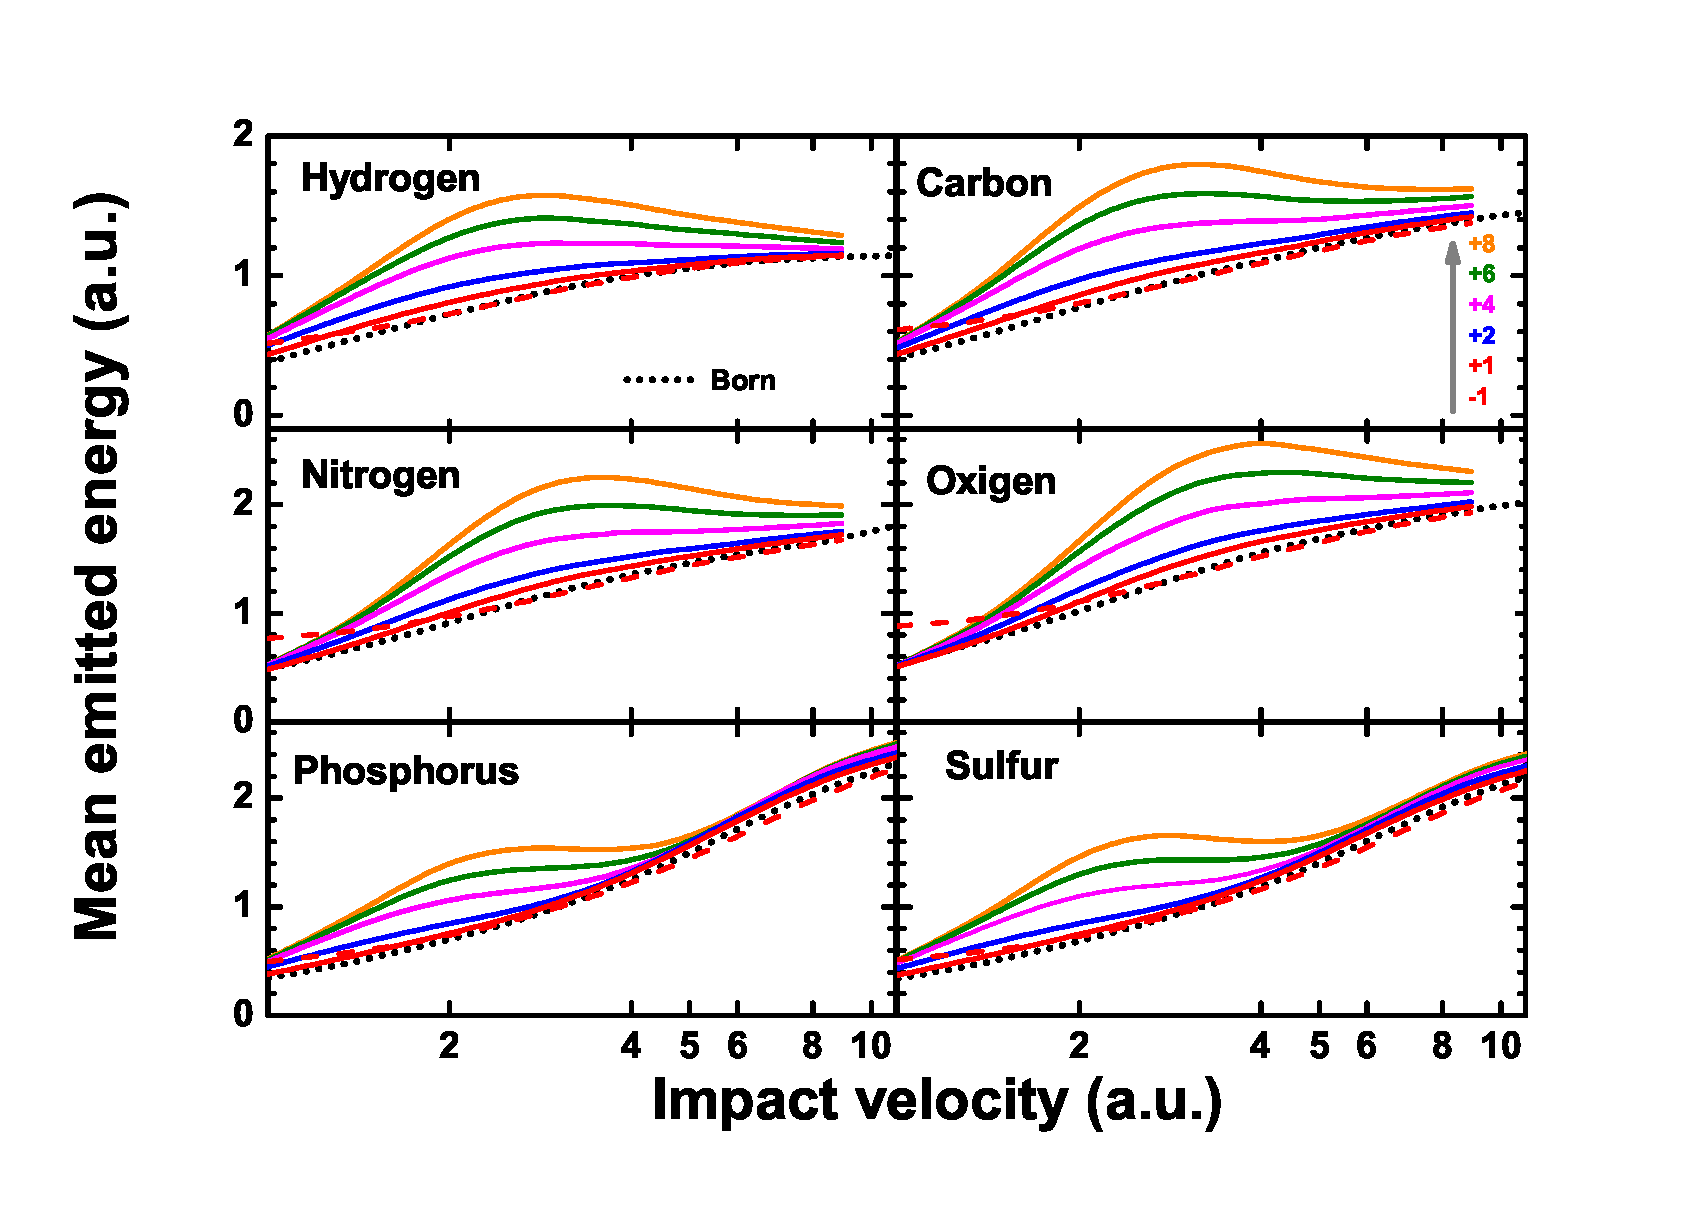
\includegraphics[width=0.75\textwidth]{figuras/Fig_finales/fig5.eps}
\caption{Mean emitted energy distribution for ionization by impact of
multicharged ions. Charge state of projectiles given by arrow.}
\label{fig:emittedener}
\end{figure} 

Figure~\ref{fig:emittedener} shows $\overline{E}_{\alpha}$ for six elements from 
Table~\ref{tab:families}. The range of impact velocities was shorten up 
to $v=10$ a.u. due to numerical limitations in the spherical harmonics 
expansion. In our theoretical treatment, we expand our final continuum 
wave function as per usual,
\begin{equation}
\psi_{\overrightarrow{k}}^{-}(\overrightarrow{r})=\sum_{l=0}^{l_{\max
}}\sum_{m=-l}^{l}R_{kl}^{-}(r)Y_{l}^{m}(\widehat{r})Y_{l}^{m^{\ast }}
(\widehat{k})\,.
\label{60}
\end{equation}
We are confident with our calculations up to $l_{\max}\sim 30$. 
As the impact velocity $v$ increases, so do $\langle E_{\alpha}\rangle$
and $l_{\max}$, which results in the inclusion of very oscillatory 
functions in the integrand. Furthermore, the integrand of
$\langle E_{\alpha}\rangle$ includes the kinetic energy $E$
(see Eq.~(\ref{40})), which cancels the small energy region and 
reinforces the large values, making the result more sensible to large
angular momenta. Regardless, for $v>10$ a.u., the first Born 
approximation holds.

In Figure~\ref{fig:emittedener} , we estimate $\overline{E}_{\alpha}$ 
in the 0.5--2 a.u.
velocity range, or equivalently from 15 to 50 eV, for all the targets.
Our results agree with the experimental findings~\cite{surdutovic2018}. 
The dependence of the mean energy value with the projectile charge $Z$ 
is surprisingly sensible, which can duplicate the proton results. 
This effect can be attributed to the depletion caused by the 
multicharged ions to the yields of low energy electrons. In the high 
approximation, surviving the $Z^{2}$ law. Then, the ratio in 
Eq.~(\ref{40}) cancels out and $\overline{E}_{\alpha}$ becomes a 
universal value independent on $Z$.

%%%%%%%%%%%%%%%%%%%%%%%%%%%%%%%%%%%%%%%%%%%%%%%%%%%%%%%%%%%%%%%%%%%%%%%%
\subsection{Emitted electron angles}
%%%%%%%%%%%%%%%%%%%%%%%%%%%%%%%%%%%%%%%%%%%%%%%%%%%%%%%%%%%%%%%%%%%%%%%%

As mentioned before, secondary electrons contribute to the total damage. 
Then, not only is the ejection energy important but also the angle 
of emission. Once again, we can consider the single differential cross 
section in terms of the ejected electron solid angle $\Omega$, 
$d\sigma_{\alpha,nl}/d\Omega$, to be expressed as a distribution function, 
and the mean angle $\overline{\theta}_{\alpha}$ can be defined as
\begin{equation}
\overline{\theta}_{\alpha}=\frac{\langle\theta_{\alpha}\rangle}
{\langle 1\rangle}=\frac{1}{\sigma_{\alpha}}\sum\limits_{nl}
\int d\Omega\,\theta\,\frac{d\sigma_{\alpha,nl}}{d\Omega}
\end{equation}

\begin{figure}[t!]
\centering
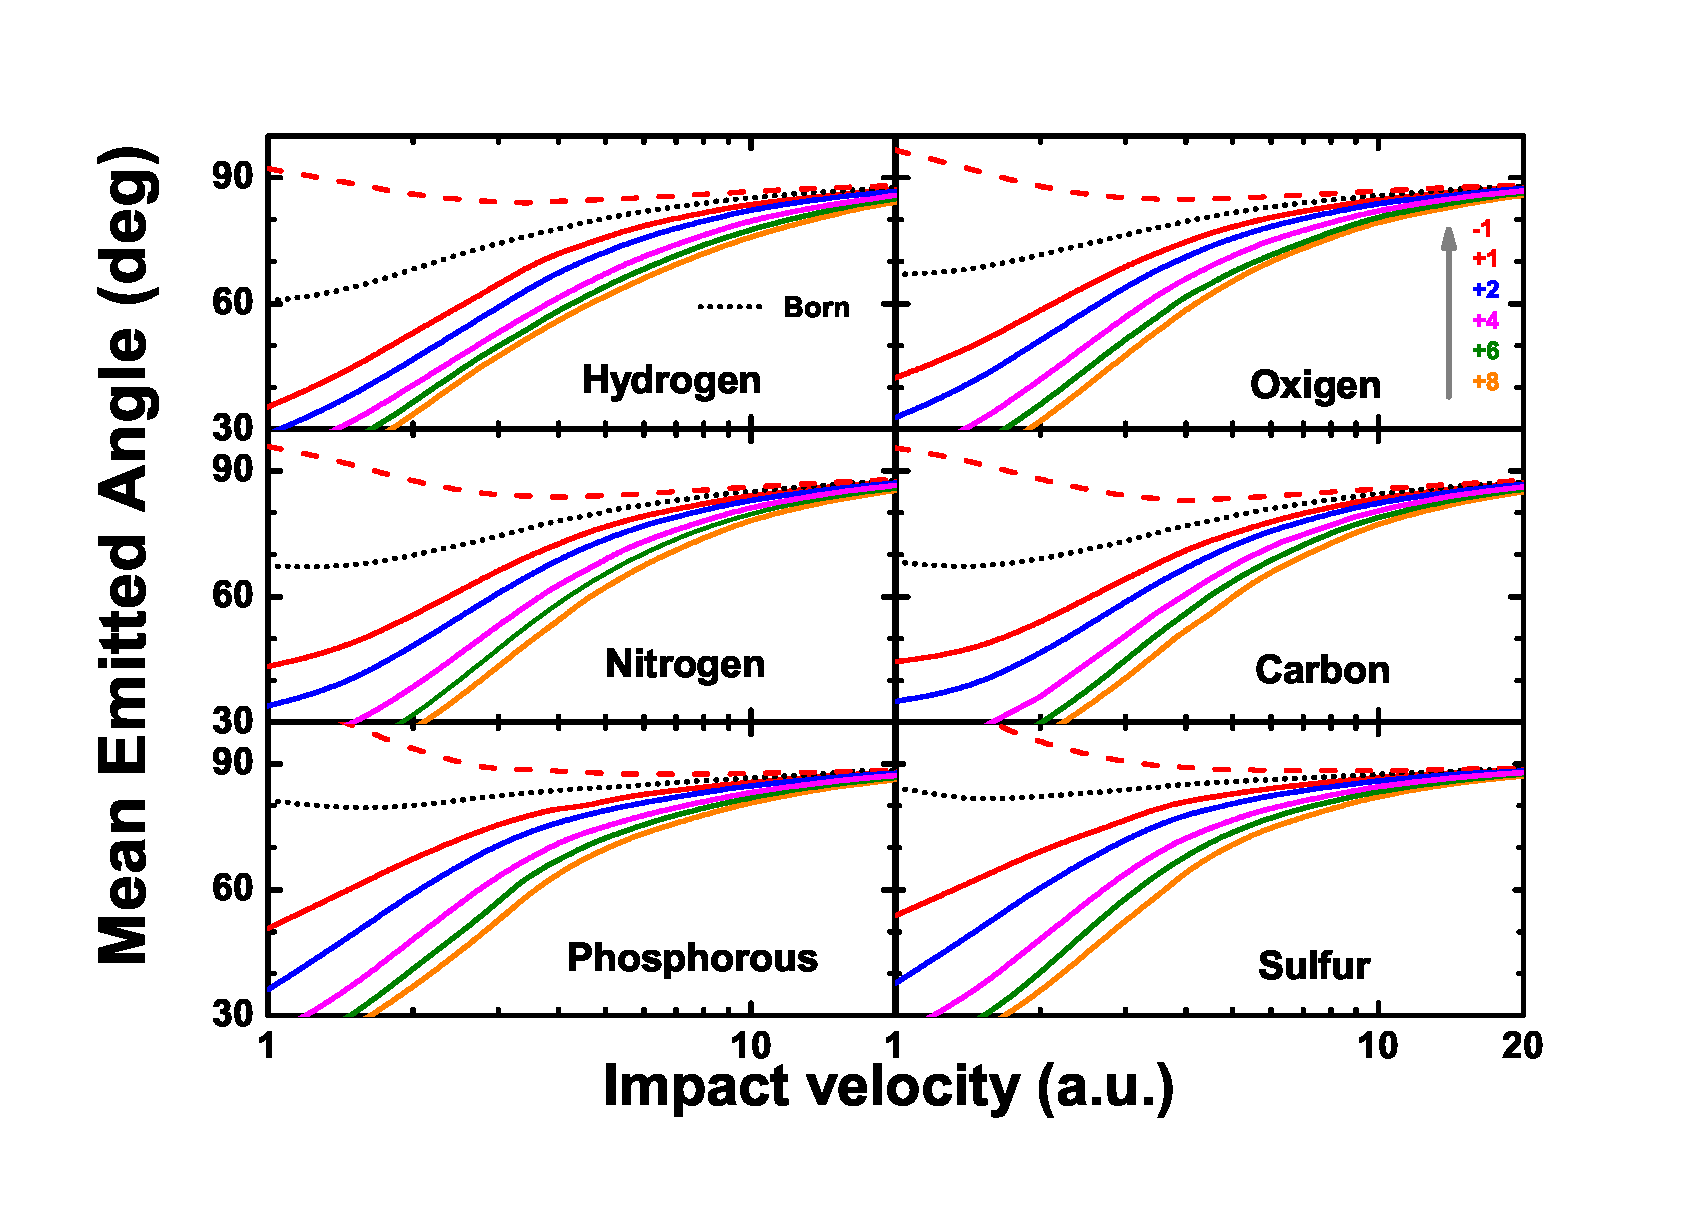
\includegraphics[width=0.75\textwidth]{figuras/Fig_finales/fig6.eps}
\caption{Mean emitted angle distribution for ionization by impact of
multicharged ions.}
\label{fig:emittedang}
\end{figure} 

Figure~\ref{fig:emittedang} shows $\overline{\theta}_{\alpha}$ for our six elements of 
interest. A new important dependence of $\overline{\theta}_{\alpha}$ 
with $Z$ is observed. It is a general belief~\cite{Rudd1992} that the 
angular dispersion of emitted electrons are nearly isotropic. This effect 
is caused by the insignificant angular anisotropy of sub-50-eV yield. 
A typical value for the ejection angle considered in the literature is 
$\overline{\theta}_{\alpha}\sim 70\degree$~\cite{surdutovic2018}, and 
it is quite correct in the range of validity of the first Born 
approximation for any target. But, when a distorted wave approximation 
is used, $\overline{\theta}_{\alpha}$ decreases substantially with $Z$ 
in the intermediate energy region, as observed in Figure~\ref{fig:emittedang}. 
For example, for C$^{+6}$ impact, the Bragg peak occurs at 0.3 MeV/amu, 
where $\overline{\theta}_{\alpha}$, computed with the CDW method, is 
about half of the value obtained with the first Born approximation. 
This correction should close the damage to the forward direction.

We can attribute this correction to the capture to the continuum effect;
the larger the charge $Z$, the smaller $\overline{\theta}$ will be. Of 
course, this effect only holds at intermediate energies and not at high 
impact energies, where the Born approximation rules. One illustrative 
observation is the behavior of antiprotons: the projectile in this case 
repels the electrons, making the distribution almost symmetric. 
Note the opposite effect of proton and antiprotons; they run one 
opposite to the other, as compared with the first Born approximation.


%%%%%%%%%%%%%%%%%%%%%%%%%%%%%%%%%%%%%%%%%%%%%%%%%%%%%%%%%%%%%%%%%%%%%%%%
\section{Ionization of Molecules}
%%%%%%%%%%%%%%%%%%%%%%%%%%%%%%%%%%%%%%%%%%%%%%%%%%%%%%%%%%%%%%%%%%%%%%%%
\subsection{The stoichiometric model}
%%%%%%%%%%%%%%%%%%%%%%%%%%%%%%%%%%%%%%%%%%%%%%%%%%%%%%%%%%%%%%%%%%%%%%%%

Lets us consider a molecule $M$ composed by $n_{\alpha}$ atoms of the
element $\alpha$, the SSM describes the total ionization cross section 
of the molecule $\sigma_{M}$ as a simple sum of ionization cross 
sections of the isolated atoms $\sigma_{\alpha}$, 
\begin{equation}
 \sigma_{M}=\sum\limits_{\alpha}n_{\alpha}\sigma_{\alpha}\,.  
 \label{eq:sumion}
\end{equation}
We divided seventeen molecular targets of our interest in three families. 
The classification defined is given in Table~\ref{tab:families}.

\begin{table}[H]
\begin{center}
\begin{tabular}{|p{0.06\textwidth}|p{0.75\textwidth}|}
\hline
 CH  & CH$_4$ (methane), C$_2$H$_2$ (acetylene), \\
     & C$_2$H$_4$ (ethene), C$_2$H$_6$ (ethane), C$_6$H$_6$ (benzene) \\
\hline
 CHN & C$_5$H$_5$N (pyridine), C$_4$H$_4$N$_2$ (pyrimidine), \\
& C$_2$H$_7$N 
(dimenthylamine), CH$_5$N (monomethylamine) \\
\hline
 \multirow{4}{*}{DNA} 
     & C$_5$H$_5$N$_5$ (adenine), C$_4$H$_5$N$_3$O (cytosine), \\
     & C$_5$H$_5$N$_5$O (guanine), C$_5$H$_6$N$_2$O$_2$ (thymine), \\
     & C$_4$H$_4$N$_2$O$_2$ (uracil), C$_4$H$_8$O (THF), \\
     & C$_5$H$_{10}$O$_5$P (DNA backbone), C$_{20}$H$_{27}$N$_7$O$_{13}$P$_2$ (dry DNA) \\
\hline
\end{tabular}
\caption{Molecular targets of our interest classified in three families.}
\label{tab:families}
\end{center}
\end{table}

We report the total ionization cross sections by the impact of 
multicharged ions for adenine, cytosine, guanine and thymine in 
Fig.~\ref{fig:crossDNA_1}. For adenine, the agreement with the 
experimental data available~\cite{iriki2011} is very good 
in our range of validity. To the best of our knowledge, there are not 
experimental data on ion--collision ionization for the rest of the 
molecules. We included electron impact measurements~\cite{rahman2016} 
with the corresponding equivelocity 
conversion for incident energies higher than 500~keV. In this region, 
the proton and electron cross section should agree. Although the electron 
impact measurements are above our findings for all the molecular targets, 
it is worth stating that our results agree very well with other 
theoretical predictions~\cite{mozejko2003,tan2018}. 
%The symbols used to make reference to the proton and electron experimental data will be kept for subsequent figures.

\begin{figure}[t!]
\centering
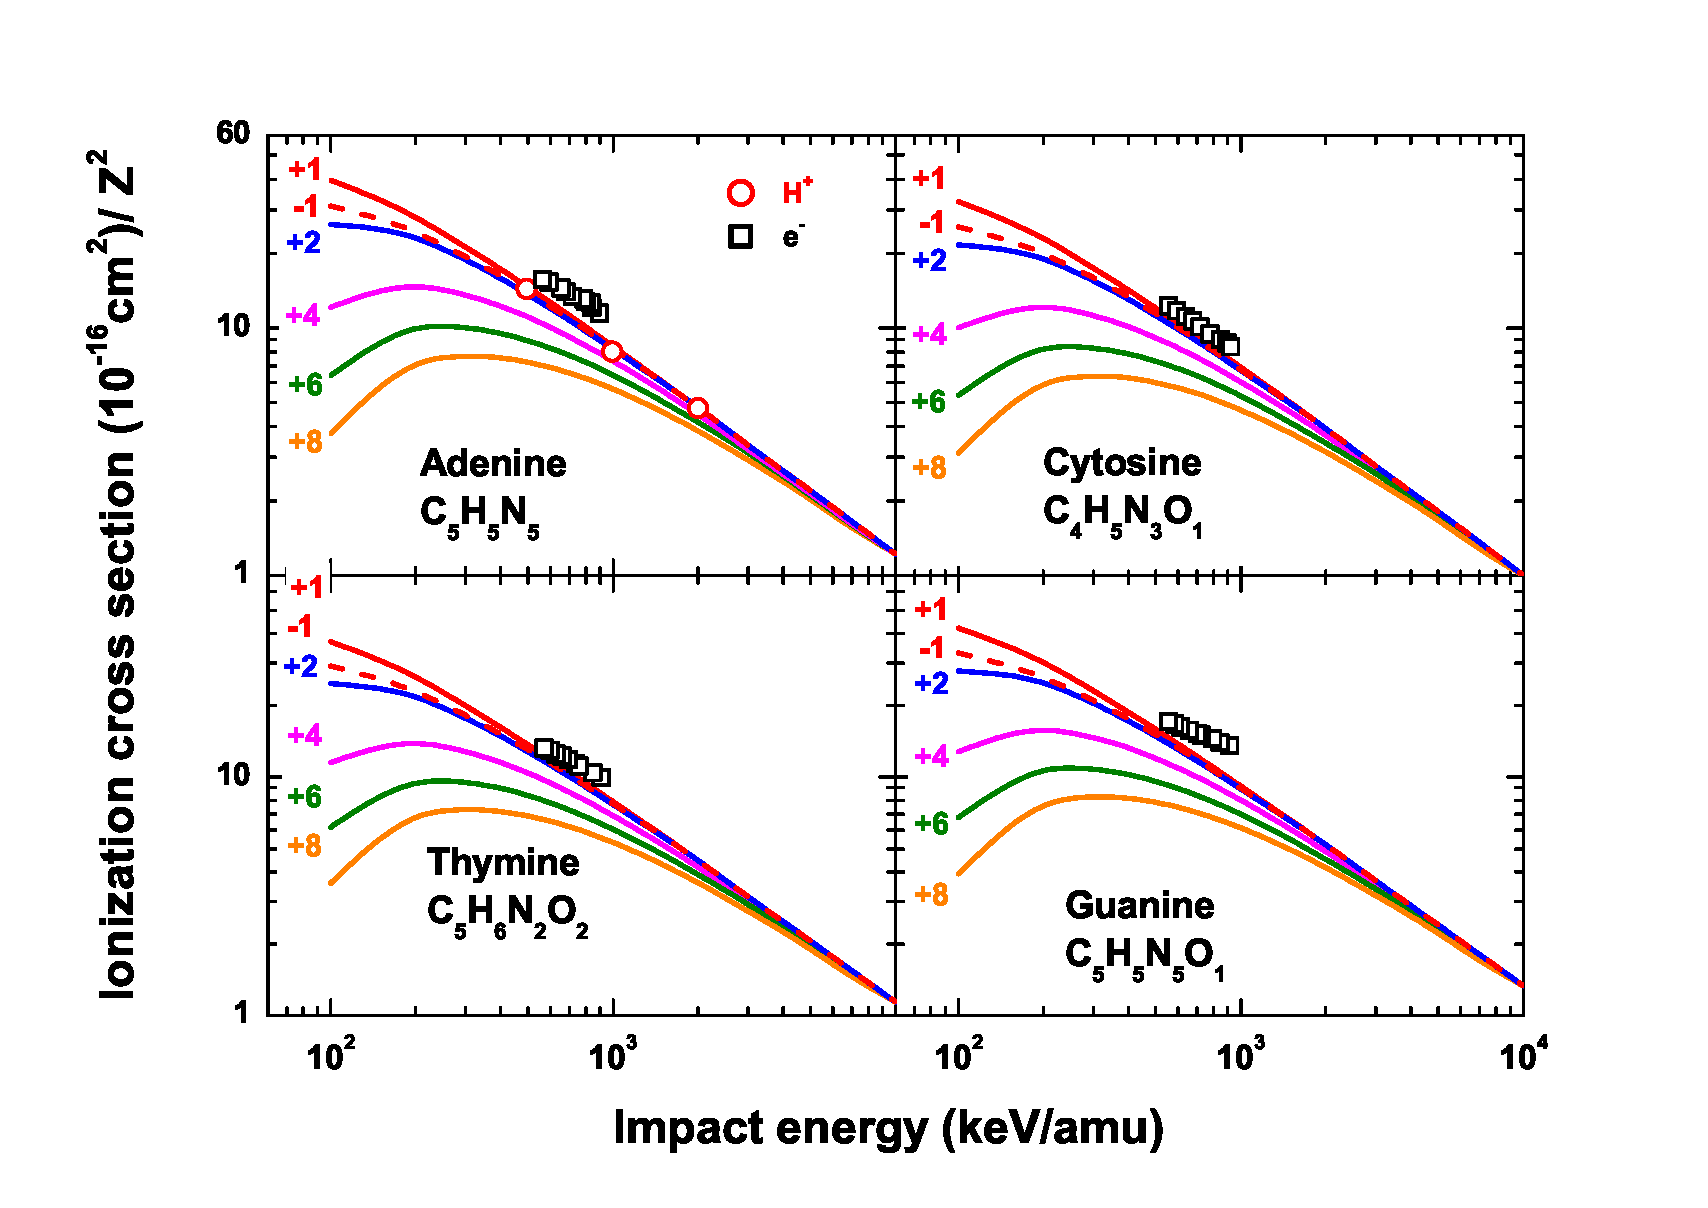
\includegraphics[width=0.75\textwidth]{figuras/Fig_finales/fig2.eps}
\caption{Scaled ionization cross section by impact of multicharged ions. 
Experiments: 
$\circ$~\cite{iriki2011} for proton impact and $\square$~\cite{rahman2016} 
for electron impact with equivelocity conversion.}
\label{fig:crossDNA_1}
\end{figure} 

Our calculations for uracil, DNA backbone, pyrimidine and THF are given in 
Fig.~\ref{fig:crossDNA_2}. 
For uracil, we have good agreement with the experimental 
proton impact measurements by Itoh~{\it et al.}~\cite{itoh2013}. 
However, for the same target, our theory fails by a factor of two for 
the experimental ionization values by the impact of 
C$^{+4}$, O$^{+6}$ and O$^{+8}$ ions~\cite{agnihotri2012,agnihotri2013}.
Nonetheless, it should be stated that our theoretical results coincide 
with calculations by Champion, Rivarola and 
collaborators~\cite{agnihotri2012,champion2012}, which may indicate a 
possible misstep of the experiments. 
For pyrimidine, we show comparison of our results with experimental data
for proton~\cite{wolff2014} and electron~\cite{bug2017} ionization. 
The electron impact measurements 
agree with our calculations for energies higher than 500keV. 
Unexpectedly, the proton impact cross sections are significantly lower 
than our findings. 
The THF molecule results are compared with proton~\cite{wang2016} 
and electron~\cite{bug2017,wolf2019,fuss2009} impact measurements, showing
overall good agreement with our theory. 

\begin{figure}[t!]
\centering
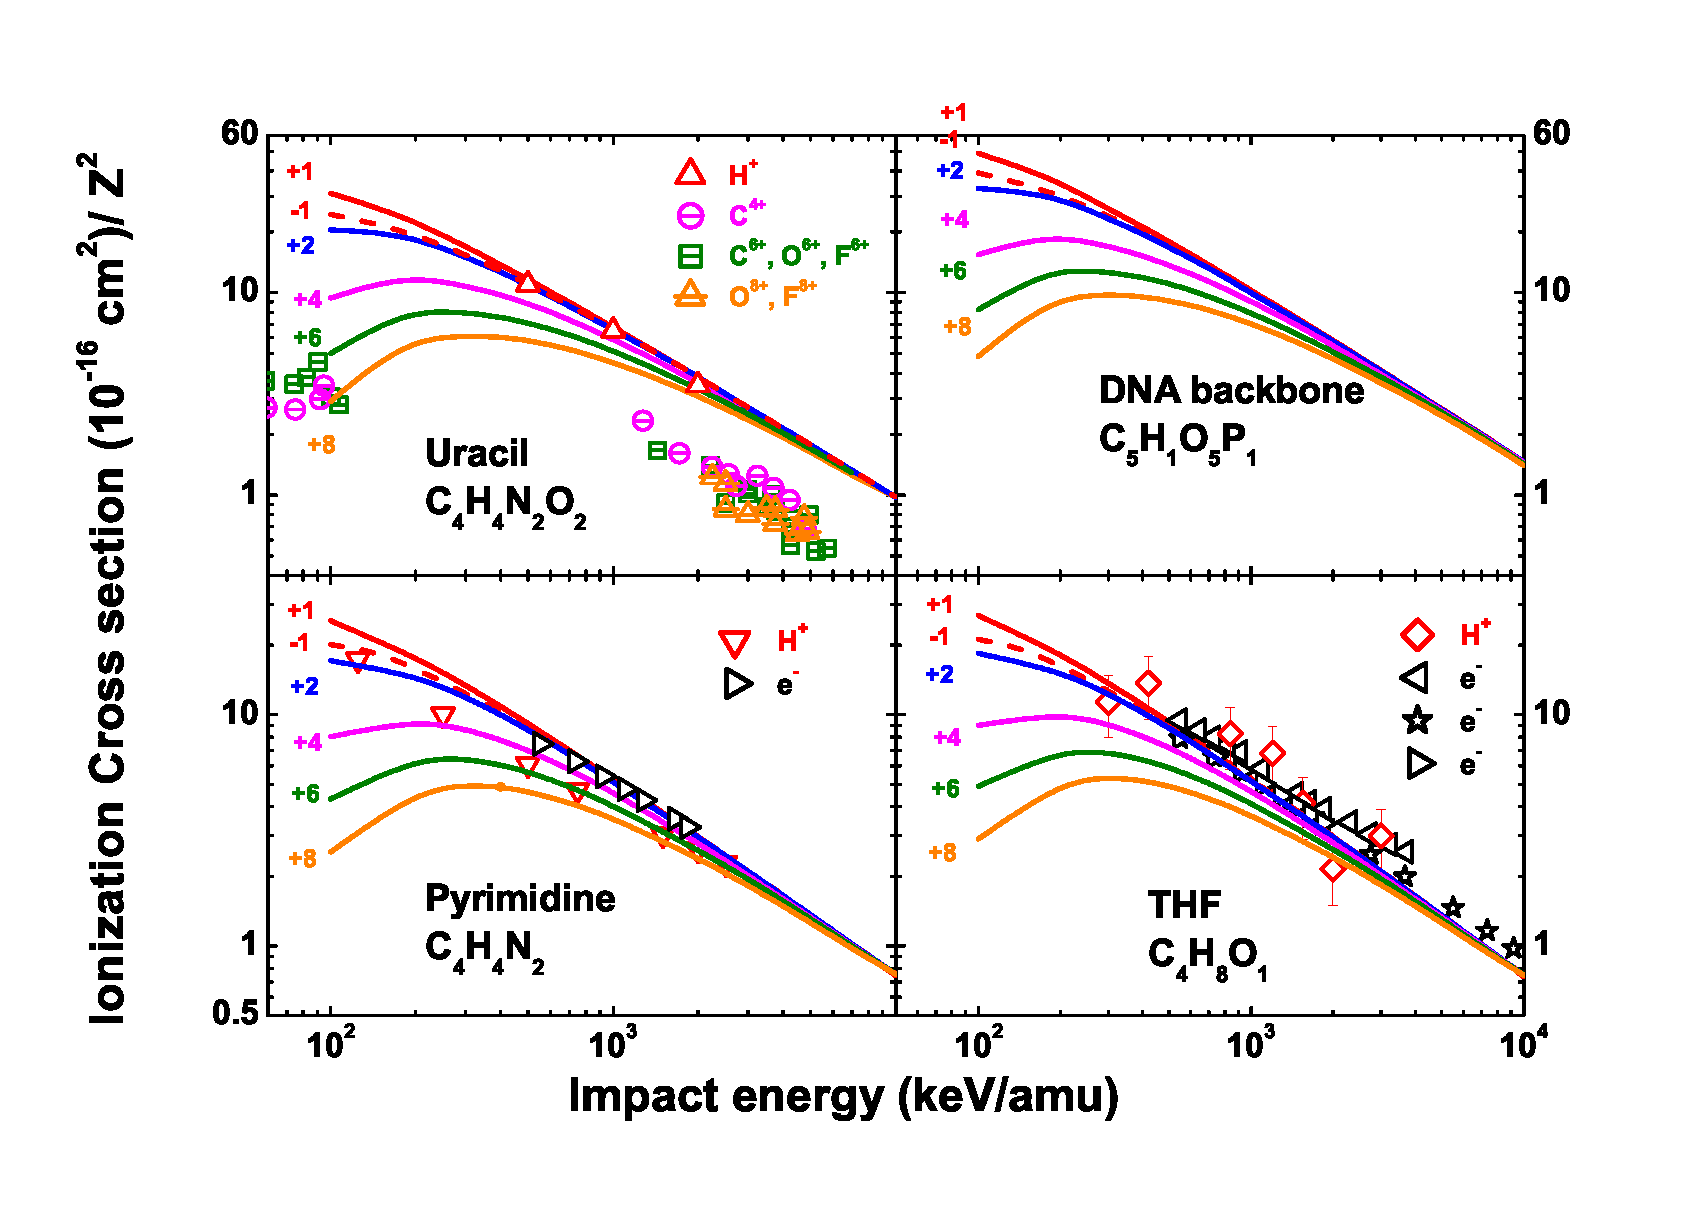
\includegraphics[width=0.75\textwidth]{figuras/Fig_finales/fig3.eps}
\caption{Scaled ionization cross section by impact of multicharged ions. 
Experiments: proton impact on $\triangle$ uracil~\cite{itoh2013}, 
$\bigtriangledown$ pyrimidine~\cite{wolff2014} and $\meddiamond$
THF~\cite{wang2016}. Impact of $\ominus$ C$^{+4}$, 
$\boxminus$ C$^{+6}$, O$^{+6}$, F$^{+6}$, and
$\triangle\mkern-14mu-$ O$^{+8}$, F$^{+8}$ on 
uracil~\cite{agnihotri2012,agnihotri2013}. 
Symbols~$\rhd$~\cite{bug2017}, $\lhd$~\cite{wolf2019}, and 
$\medstar$~\cite{fuss2009} for electron impact with equivelocity conversion.}
\label{fig:crossDNA_2}
\end{figure} 

%%%%%%%%%%%%%%%%%%%%%%%%%%%%%%%%%%%%%%%%%%%%%%%%%%%%%%%%%%%%%%%%%%%%%%%%
\subsection{Scaling rule}
%%%%%%%%%%%%%%%%%%%%%%%%%%%%%%%%%%%%%%%%%%%%%%%%%%%%%%%%%%%%%%%%%%%%%%%%
\subsubsection{Toburen numbers}
%%%%%%%%%%%%%%%%%%%%%%%%%%%%%%%%%%%%%%%%%%%%%%%%%%%%%%%%%%%%%%%%%%%%%%%%

The first attempt to develop a comprehensive but straightforward 
phenomenological model for electron ejection from large molecules was 
proposed by Toburen {\it et al.}~\cite{toburen1975,toburen1976}. 
The authors found it convenient to scale the experimental ionization 
cross section in terms of the number of active or weakly--bound valence 
electrons $n_e$ (i.e. total number of electrons minus the K--shell).
Following Toburen, we can define the ionization cross section per weakly 
bound electron, $\sigma_{e}^T$, as
\begin{equation}
\sigma_{e}^T=\frac{\sigma_{M}}{n_e}=\frac{\sum\limits_{\alpha}
n_{\alpha}\sigma_{\alpha}}{\sum\limits_{\alpha}n_{\alpha}\nu_{\alpha}^T}
=\sigma_{e}^T(v)\,, 
\label{27} 
\end{equation}
where $\nu_{\alpha}^T$ are the Toburen numbers for each $\alpha$ atom 
is given by
\begin{equation}
\nu_{\alpha}^T=\left\{ 
\begin{array}{ll}
1, & \text{for H,} \\
4, & \text{for C,} \\ 
5, & \text{for N and P,} \\ 
6, & \text{for O and S}\,.
\end{array}\right.
\label{eq:nelec} 
\end{equation} 
The Toburen rule can be stated by saying that 
$\sigma_{e}$ is a \textit{universal} parameter independent on the 
molecule, which depends solely on the impact velocity, and holds for 
high impact energies (i.e. 0.25--5 Mev/amu).
These $\nu_{\alpha}^T$ can be interpreted as the number of active 
electrons in the collision. Of course, at very high energies also de 
K--shell electrons will be ionized and these numbers will be different.
A similar dependence with the number of weakly bound electrons was 
found in Ref.~\cite{itoh2013} for proton impact on uracil and adenine.

\begin{figure}[t!]
\centering
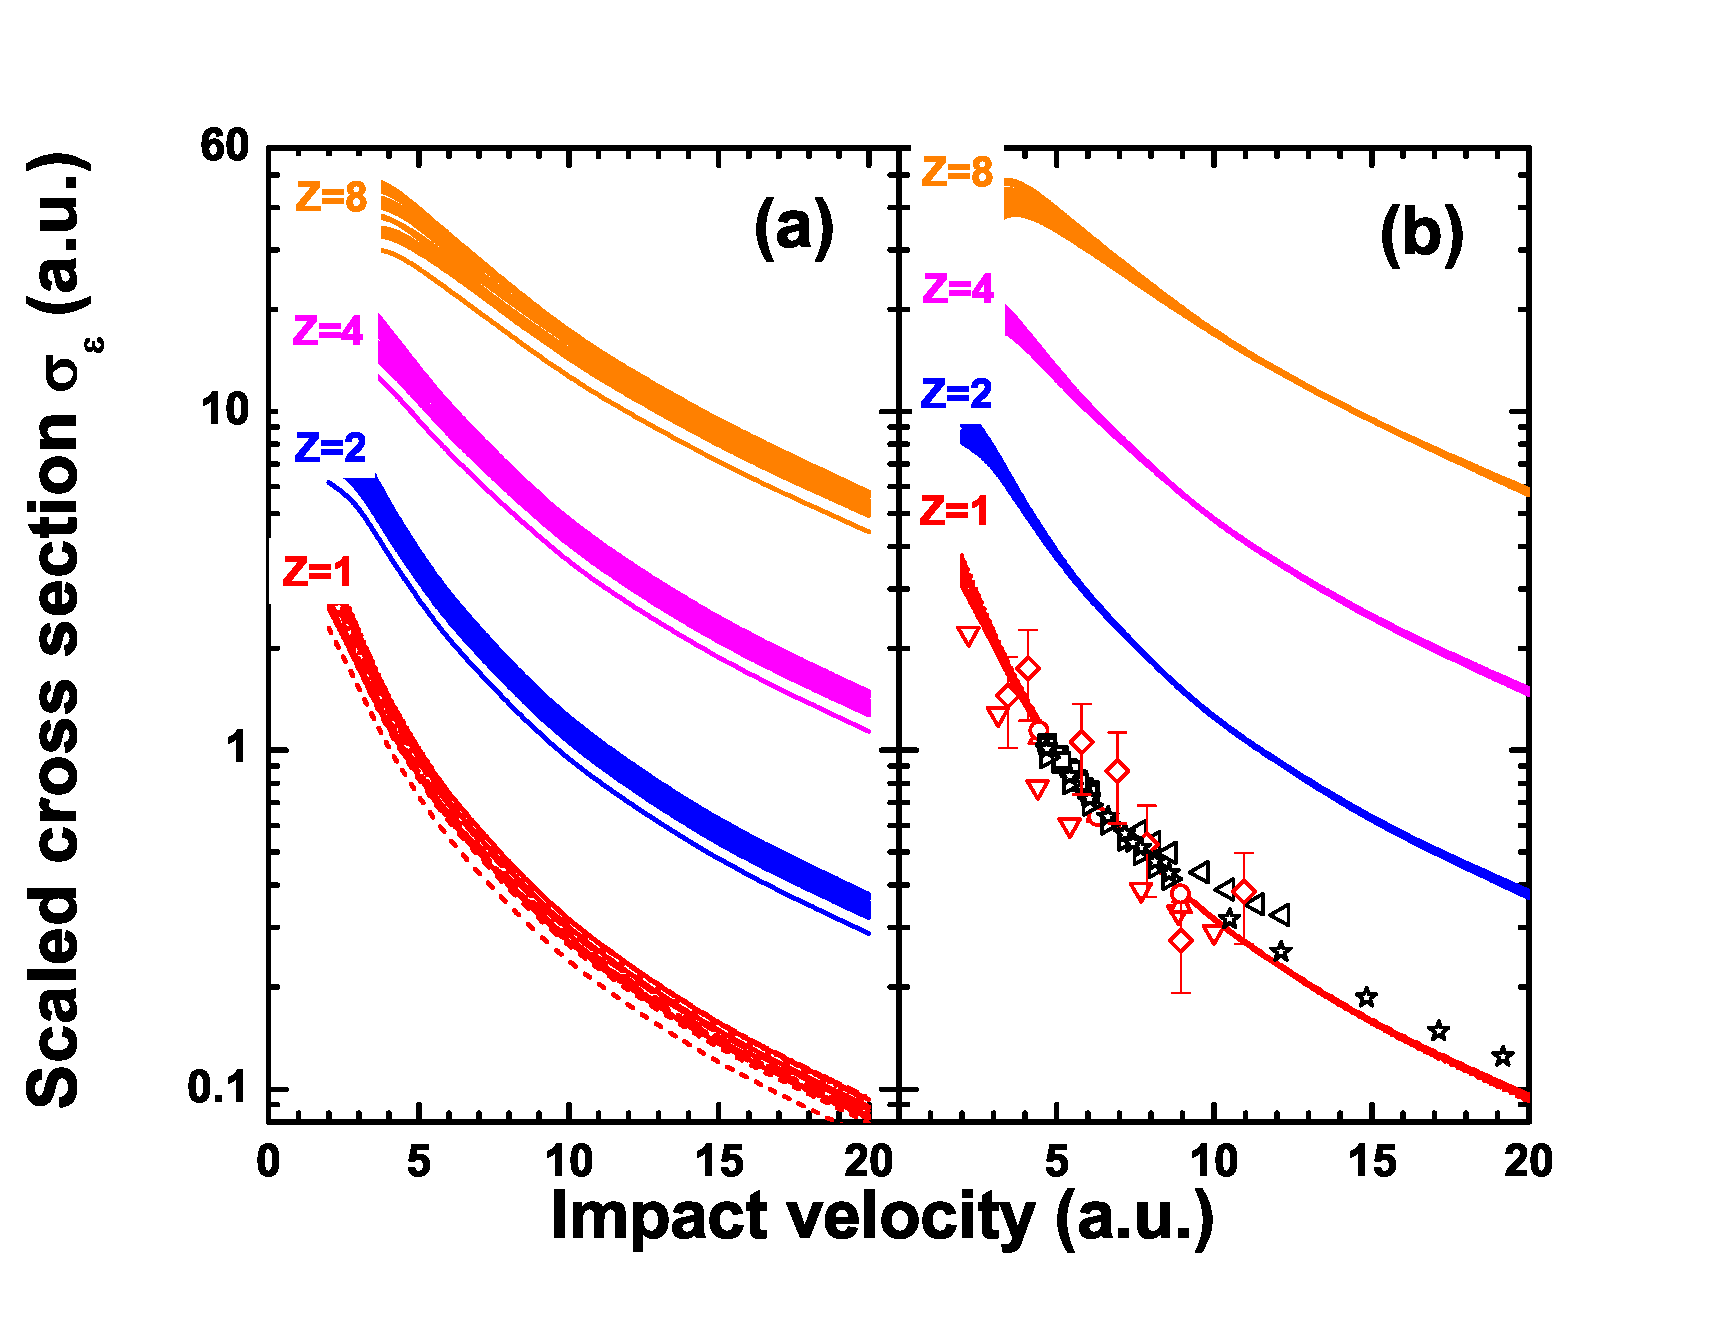
\includegraphics[width=0.75\textwidth]{figuras/Fig_finales/fig4.eps}
\caption{Scaled ionization cross section per weakly bound electron using
(a)~the Toburen numbers $\nu_{\alpha}^T$, and (b) our proposed numbers
$\nu_{\alpha}^{\text{CDW}}$. Experiments: proton impact on 
$\circ$ adenine~\cite{iriki2011}, $\triangle$ uracil~\cite{itoh2013}, 
$\bigtriangledown$ pyrimidine~\cite{wolff2014} and $\meddiamond$ 
THF~\cite{wang2016}; electron impact on $\rhd$ pyrimidine~\cite{bug2017},
and $\lhd$, $\medstar$~\cite{wolf2019,fuss2009} THF.}
\label{fig:newscaling}
\end{figure}

Our CDW results for $\sigma_{e}^T$ are shown in 
Fig.~\ref{fig:newscaling}a as a function of 
the impact energy for different projectile charges computed with the 
SSM for the molecular targets from Table~\ref{tab:families}. 
The universality with $Z$ is the one provided 
by Born approximation, i.e., $\sigma_{e}^T(Z)=Z^{2}\sigma_{e}^T(Z=1)$, 
and it holds for large impact velocities, as shown 
Fig.~\ref{fig:newscaling}a.
Of course, for lower impact velocities, the CDW breaks the behavior of 
the $Z^{2}$ rule. Although the Toburen scaling holds for high energies, 
its performance is still not satisfactory: the universal band is quite 
broad. 

%%%%%%%%%%%%%%%%%%%%%%%%%%%%%%%%%%%%%%%%%%%%%%%%%%%%%%%%%%%%%%%%%%%%%%%%
\subsubsection{New scaling}
%%%%%%%%%%%%%%%%%%%%%%%%%%%%%%%%%%%%%%%%%%%%%%%%%%%%%%%%%%%%%%%%%%%%%%%%

The departure of our theoretical 
results from the Toburen rule can be easily understood %explained by the fact that 
%our atomic cross sections $\sigma_{\alpha}$ behave differently for 
%each atom in terms of the projectile charges. By 
by inspecting Fig.~\ref{fig:atomscaling}. It can be noted that the 
rule $\sigma_{\alpha}/\nu_{\alpha}^T\sim \sigma_{e}^T$, approximatelly 
constant, is not well satisfied by the CDW. 
For example, Fig.~\ref{fig:atomscaling} shows that the cross sections
for O are actually very similar to the cross sections for C, suggesting 
4 active electrons in O instead of 6. In the same way, the number of
active electrons for N, P and S are also different from the 
$\nu_{\alpha}^T$ of Eq.~(\ref{eq:nelec}). 

Based on the CDW results, we propose a new scaling,
\begin{equation}
\sigma_{e}=\frac{\sigma_M}{\sum\limits_{\alpha}n_{\alpha}
\nu_{\alpha}^{\text{CDW}}},
\label{32} 
\end{equation}
where $\sigma_M$ follows Eq.~(\ref{eq:sumion}), and 
$\nu_{\alpha}^{\text{CDW}}$ are the new active--electron numbers 
per atom obtained from the CDW ionization cross sections for 
different ions in H, C, N, O, P , and S targets. 
Our proposed active--electron numbers are
\begin{equation}
\nu_{\alpha }^{\text{CDW}} \sim\left\{ 
\begin{array}{ll}
1, & \text{for H,} \\
4, & \text{for C, N, and O,} \\ 
4.5, & \text{for P and S}\,.
\end{array}
\right. 
\label{eq:scalingCDW}
\end{equation}

The new scaled cross sections $\sigma_{e}$ are plotted in Figure~4b. 
A much better sharp band is observed, especially for impact energies 
$E=(0.5-8)$~MeV/amu for $Z=1$ and $Z=2$, and $E=(2.5-8)$~MeV/amu for 
$Z>2$. In fact, the experimental data for ionization of 
adenine~\cite{iriki2011}, uracil~\cite{itoh2013}, 
pyrimidine~\cite{wolff2014} and THF~\cite{wang2016} by proton impact 
seems to corroborate the new scaling. 
We also included the electron impact ionization measurements with equivelocity 
conversion on pyrimidine~\cite{bug2017}, and THF~\cite{bug2017,wolf2019,fuss2009}. 
It will be interesting to cross--check for experiments with higher 
projectile charge states. 

\begin{table}[H]
\begin{center}
\begin{tabular}{|ll|ll|ll|}
\hline
 Molecule & $n_e$ &Molecule         & $n_e$ & Molecule             & $n_e$ \\
\hline
 H$_2$    & 2  & C$_2$H$_7$N         & 19    & C$_4$H$_5$N$_3$O     & 37    \\
 H$_2$O   & 6  & C$_4$H$_8$O         & 28    & C$_5$H$_6$N$_2$O$_2$ & 42    \\
 NH$_3$   & 7  & C$_4$H$_4$N$_2$     & 28    & C$_5$H$_5$N$_5$      & 45    \\
 CH$_4$   & 8  & C$_6$H$_6$          & 30    & C$_5$H$_5$N$_5$O     & 49    \\
 CH$_5$N  & 13 & C$_4$H$_4$N$_2$O$_2$& 36    & C$_5$H$_{10}$O$_5$P  & 54.5  \\
 \hline
\end{tabular}
\caption{New scaling numbers for some molecular targets of biological interest.}
\label{nn}
\end{center}
\end{table}

By using Eq.~(\ref{eq:scalingCDW}), the number of active electrons 
$n_e=\sum_{\alpha} n_{\alpha} \nu_{\alpha}^{\text{CDW}}$ can be redefined. 
We give new values in Table~\ref{nn} for some molecules of interest.
These values are very different from the ones proposed by Toburen and used by 
other authors~\cite{itoh2013}.
Moreover, an alternative way of showing the scaling can be attained by 
plotting the ionization cross sections of molecules as a function of the 
number of active electrons from Table~\ref{nn}. Our findings are displayed 
in Fig.~\ref{fig:recta} for impact energies 0.5, 1 and 2 MeV. As can be 
noted, the computed CDW ionization cross sections for all the molecules  
show a linear dependence with the number of electrons from Table~\ref{nn}. 
We obtain similar results even for $E=10$~MeV. The comparison with the 
experimental data available shows very nice agreement, from the smallest 
molecules, H$_2$, H$_2$O and CH$_4$, up to the most complex ones, like 
adenine or guanine. In some cases, the experimental data were interpolated.
Care was taken in such procedure.

\begin{figure}[t!]
\centering
\includegraphics[width=0.75\textwidth]{figuras/Fig_finales/fig_recta.eps}
\caption{Ionization cross sections by impact of protons at 0.5, 1 and 2 MeV
in terms of the number of active electrons given by Table~\ref{nn}.
Experiments: $\circ$~adenine~\cite{iriki2011}, $\triangle$ uracil~\cite{itoh2013}, 
$\bigtriangledown$ pyrimidine~\cite{wolff2014}, 
$\blacktriangle$ C2H$_7$N, CH$_5$N, methane and amonia~\cite{lynch1976},
$\bigstar$ amonia and H$_2$~\cite{rudd1985}, and $\bullet$ water~\cite{luna2007}.}
\label{fig:recta}
\end{figure}

%%%%%%%%%%%%%%%%%%%%%%%%%%%%%%%%%%%%%%%%%%%%%%%%%%%%%%%%%%%%%%%%%%%%%%%%
\subsection{A modified stoichiometric model}
%%%%%%%%%%%%%%%%%%%%%%%%%%%%%%%%%%%%%%%%%%%%%%%%%%%%%%%%%%%%%%%%%%%%%%%%

The SSM considers the molecule to be assembled by isolated neutral atoms, 
which is definitively unrealistic. A first improvement can be suggested 
by assuming that the atoms are not neutral and that they have an uneven
distribution of electrons within the molecule; this distribution can be
given by an effective charge $q_{\alpha}$. A possible value for 
$q_{\alpha}$ is given by the Mulliken charge. However, there are a wide
variety of charge distributions, such as the net or natural atomic
charge~\cite{lee2003}, the L\"owdin charge, etc.

Consider that the total amount of electrons $Q_{\alpha }$ on the element
$\alpha$ are equally distributed on all the $\alpha$ atoms. Therefore, 
each element $\alpha$ will have an additional charge: 
$q_{\alpha}=Q_{\alpha}/n_{\alpha}$, which can be positive or negative.
This value will depend on the relative electronegativity value with 
respect to the other atoms~\cite{rappe1991}. Now, instead of an
integer number of elements $n_{\alpha}$ of the atom $\alpha$, we have a 
fractional number of atoms given by 
\begin{equation}
n_{\alpha }^{\prime }=n_{\alpha }-
\frac{q_{\alpha }}{\nu_{\alpha }^{\text{CDW}}}
\label{eq:newstoi}
\end{equation}%
In the case of neutral atoms, $q_{\alpha}=0$ and we recover 
$n_{\alpha}^{\prime}=n_{\alpha}$, as it should be.

To inspect the effect of $q_{\alpha}$, we computed the molecular
structure of several nucleobases with the {\sc gamess} code. We 
used the 6-31G(d,p) basis set, which includes polarization 
functions for all the atoms. The calculations were carried out 
implementing the B3LYP functional~\cite{Becke1993,Stephens1994} to 
account for the correlation and exchange effects. 
In Table~\ref{tab:newstoi}, we display the charge $q_{\alpha}$ of four 
DNA molecules. 

\begin{table}[H]
\begin{center}
\begin{tabular}{|p{0.12\textwidth}|p{0.07\textwidth}|p{0.07\textwidth}|p{
0.07\textwidth}|p{0.07\textwidth}|p{0.25\textwidth}|}
\hline
Element & C & H & N & O & New stoichiometry \\
\hline
Adenine & +0.32 & +0.23 & --0.55 &       & 
C$_{4.92}$H$_{4.77}$N$_{5.14}$ \\ 
\hline
Cytosine & +0.28 & +0.21 & --0.56 & --0.53 & 
C$_{3.93}$H$_{2.79}$N$_{5.14}$O$_{1.13}$ \\ 
\hline
Guanine & +0.46 & +0.20 & --0.58 & --0.36 & 
C$_{4.89}$H$_{4.80}$N$_{5.15}$O$_{1.09}$ \\ 
\hline
Thymine & +0.20 & +0.19 & --0.54 & --0.52 & 
C$_{4.95}$H$_{1.95}$N$_{6.13}$O$_{2.13}$ \\ 
\hline
\end{tabular}
\caption{Effective charge $q_{\alpha}$ and new stoichiometric formula 
defined by Eq.~(\ref{eq:newstoi}) for four DNA molecules.}
\label{tab:newstoi}
\end{center}
\end{table}

\begin{figure}[t!]
\centering
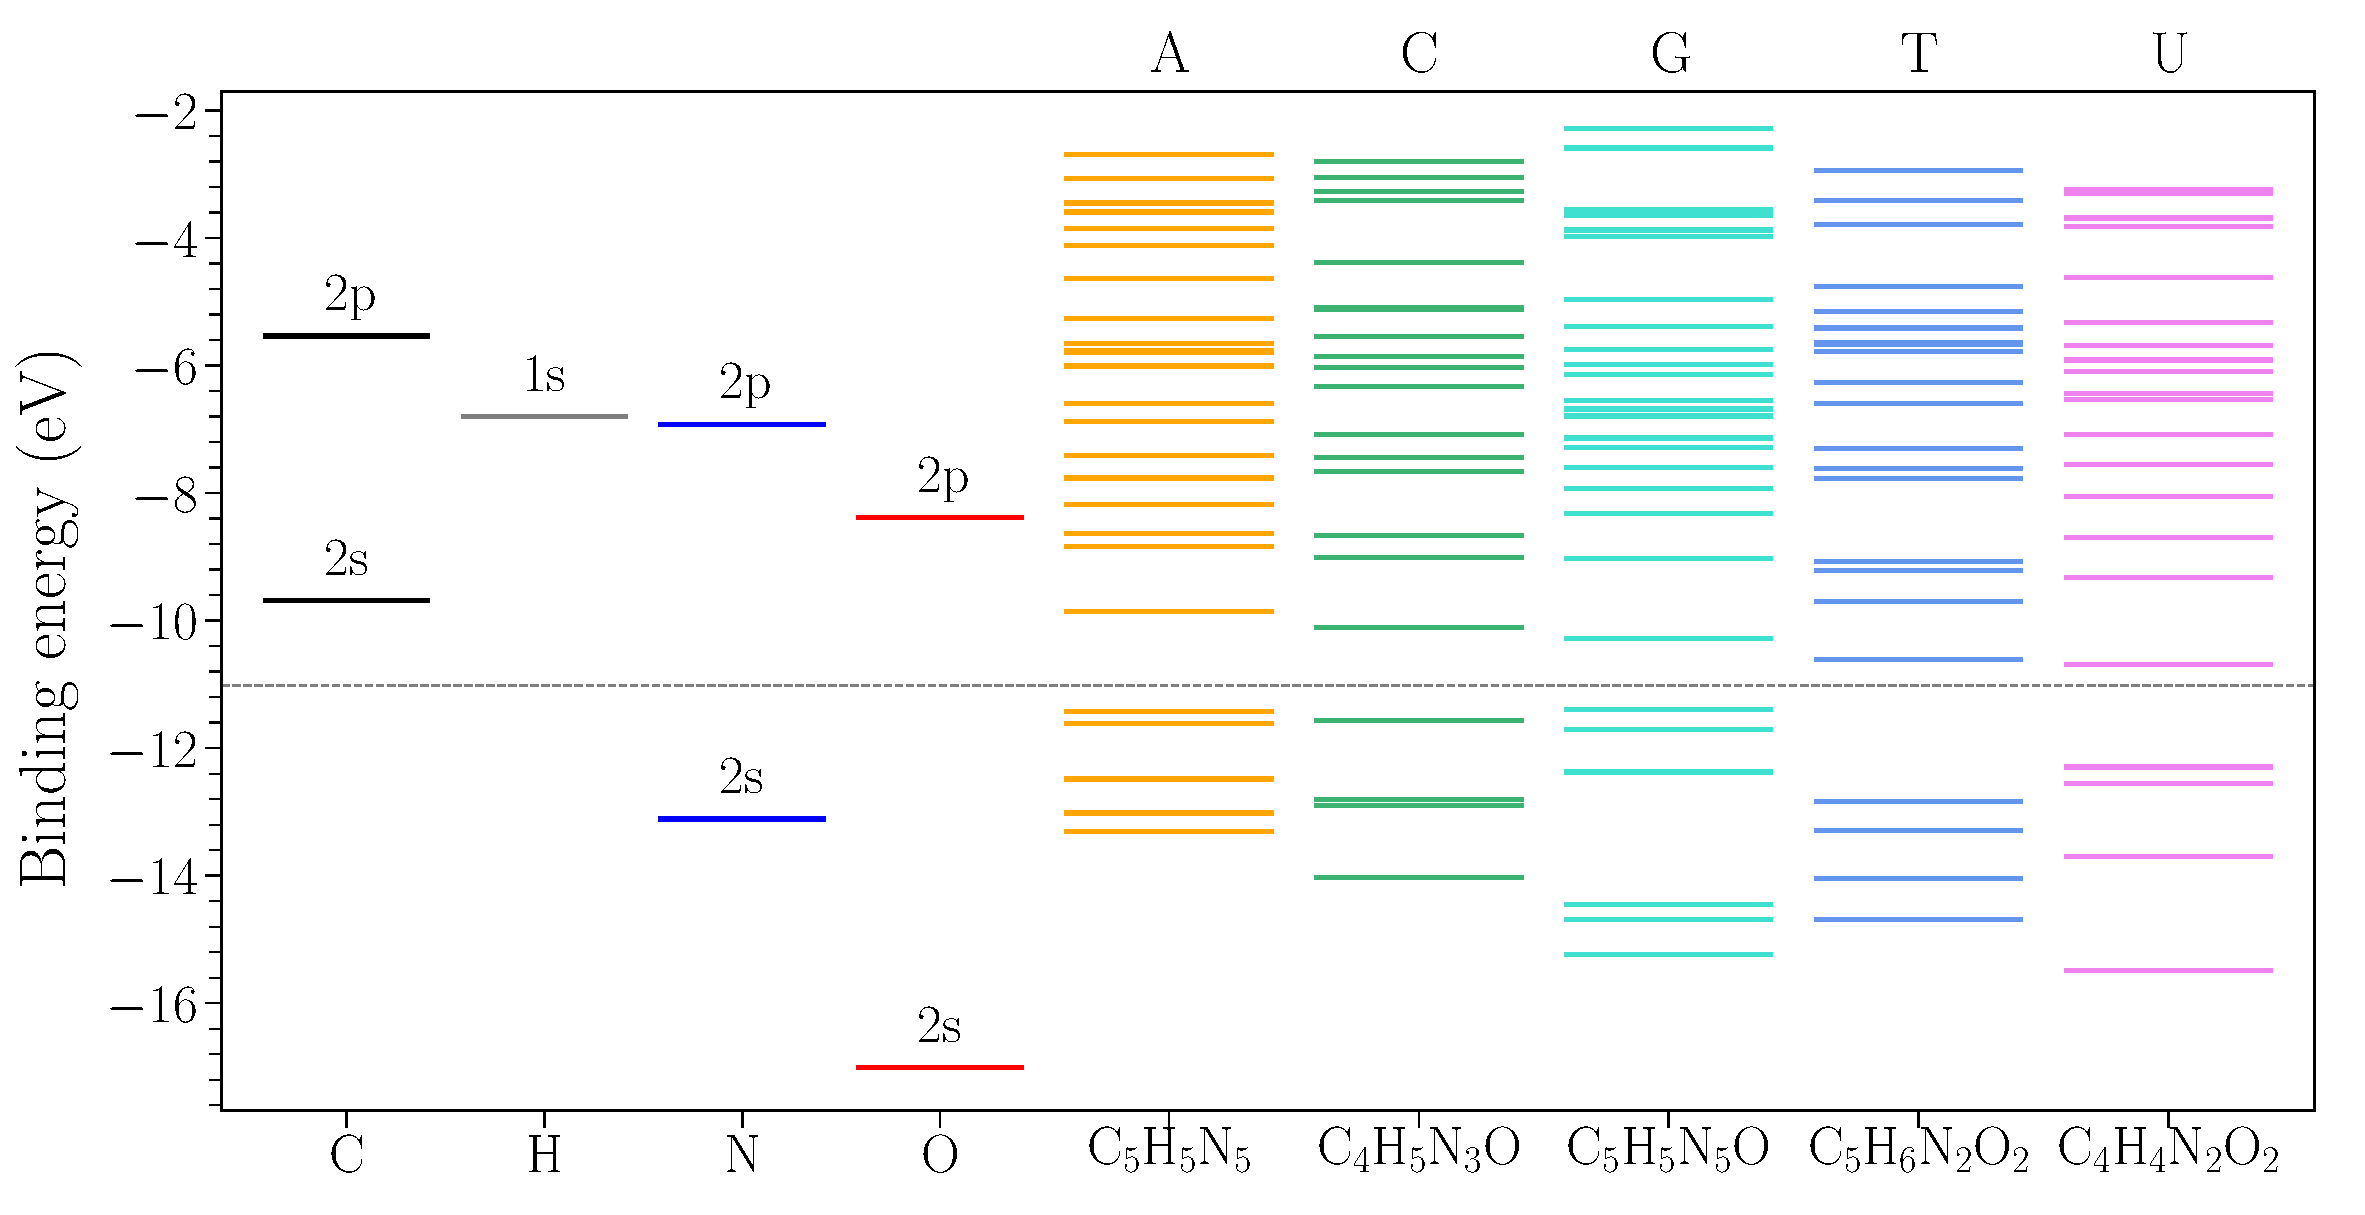
\includegraphics[width=\textwidth]{figuras/levelsDNA.eps}
\caption{Theoretical molecular binding energies for adenine, cytosine, 
guanine, thymine and uracil compared to those of atomic constituents.}
\label{fig:bindener}
\end{figure}

The molecular binding energies of the outer electrons for adenine, 
cytosine, guanine and thymine are shown in Fig.~\ref{fig:bindener}. 
On the left side of the figure, we show the atomic Hartree--Fock energies 
of the constituent elements, which can give an idea of how the molecular 
levels distribute. A dashed line around $-0.8$~a.u. is drawn to separate 
in two the band levels of the outer electrons. The electrons in the molecular 
targets corresponding to the $2s$ of N and C in the atomic case are 
placed in a secondary gap. The lower levels of the secondary gap 
correspond to the oxygen. The number of electrons in the valence 
shell for all O would seem to be equal to 4, as previously setted by the 
scaling rule Eq.~(\ref{eq:scalingCDW}). The N case is not as 
straightfoward; the electrons that would correspond to the $2s$ are 
located just below the line. The $\nu_{\alpha }^{\text{CDW}}$ value 
given for N would suggest that a significant amount of electron density 
from the secondary gap is shared with the valence band.

\begin{table}[H]
\begin{center}
\begin{tabular}{llllll}
\hline
 $E_{\text{av}}$ & Adenine & Cytosine & Guanine & Thymine & Uracil \\
\hline
 Molecular & -7.1955 & -6.9058 & -7.4725 & -7.5304 & -7.6224 \\
 Toburen   & -8.4236 & -8.6743 & -8.7275 & -8.7947 & -9.0022 \\
 Our work  & -7.9027 & -7.8639 & -7.9420 & -7.8066 & -7.8839 \\
\hline
\end{tabular}
\caption{.}
\label{tab:gravener}
\end{center}
\end{table}


By implementing Eq.~(\ref{eq:newstoi}), it is possible to determine a 
new stoichiometric formula (last column of Table~\ref{tab:newstoi}). 
Now, instead of having an integer number of atoms $n_{\alpha}$, we obtain 
a fractional number $n_{\alpha}^{\prime}$. 
Molecular cross sections $\sigma^{\prime}$ can be computed considering 
such values. Relative errors for the ionization cross sections were 
computed for the DNA bases from Table~\ref{tab:newstoi}. The differences 
obtained were of just very few percents, which indicates that the modified 
SSM is a quite robust model to handle these type of molecule within 
the range error expected for this model.

%%%%%%%%%%%%%%%%%%%%%%%%%%%%%%%%%%%%%%%%%%%%%%%%%%%%%%%%%%%%%%%%%%%%%%%%
\section{Conclusions}
%%%%%%%%%%%%%%%%%%%%%%%%%%%%%%%%%%%%%%%%%%%%%%%%%%%%%%%%%%%%%%%%%%%%%%%%

We calculated ionization cross sections by impact of antiprotons, 
H$^{+}$, He$^{+2}$, Be$^{+4}$, C$^{+6}$, and O$^{+8}$ for seventeen 
molecules containing H, C, N, O, P and S with the CDW method. The 
importance of the influence of $Z$ was observed in the mean energy 
$\overline{E}_{\alpha}$ and angle $\overline{\theta}_{\alpha}$. 
For a given target $\alpha$, as the nuclear charge of the projectile 
$Z$ increases, so does the mean energy of emittion $\overline{E}_{\alpha}$. 
Conversely, the mean angle of emission  $\overline{\theta}_{\alpha}$ 
decreases. At high impact energy, say larger than 1 MeV/amu, these 
values converge to the Born approximation, which embodies the simple 
$Z^{2}$ law. The seventeen molecules selected were investigated using 
the simple stoichiometric model. Results for eigth DNA bases were 
presented and compared with the sparse available experiments. We explore 
the rule of Toburen which scales all the molecular ionization cross 
section when divided by the number of weakly bound valence electrons 
$\nu_{\alpha}^T$ given by Eq.~(\ref{27}). 
We found the rule scales much better when normalizing our theoretical 
ionization cross sections to the number $\nu_{\alpha}^{\text{CDW}}$ 
given by Eq.~(\ref{eq:scalingCDW}). Finally, we attempt to improve the 
stoichiometric model by using the Mulliken charge to define a new model 
containing fractional rather than integer proportions. No substantial 
correction was found, which indicates that our modified SSM works quite 
well. By inspecting the molecular binding energy from quantum mechanical 
structure calculations, we were able to understand the values defined
for $\nu_{\alpha}^{\text{CDW}}$.

The main objective of this article is to provide the tools to estimate 
any inelastic parameter parameter --such as emission angle, emitted mean 
energy and cross section-- by the impact of any multicharged on any 
molecule containing H, C, N, O, P and S, with the help of the 
stoichimetrical model. Our goal was quite ambitious, considering the 
simplicity of our proposal. However, we think our results could be used 
to estimate the ionization magnitude with an acceptable level of 
uncertainty.

\bigskip

\begin{thebibliography}{99}

\bibitem{gamess}
M. W. Schmidt, K. K. Baldridge, J. A. Boatz, S. T. Elbert, M. S. Gordon, 
J. H. Jensen, S. Koseki, N. Matsunaga, K. A. Nguyen, S. J. Su, T. L. Windus, 
M. Dupuis, J. A. Montgomery 
J. Comput. Chem. 14, 1347-1363 (1993)

\bibitem{miraglia2008} 
J. E. Miraglia and M. S. Gravielle. Ionization of the
He, Ne, Ar, Kr, and Xe isoelectronic series by proton impact. 
Phys Rev A \textbf{78}, 052705 (2008)

\bibitem{miraglia2009} 
J. E. Miraglia, Ionization of He, Ne, Ar, Kr, and Xe
by proton impact: Single differential distributions. 
Phys. Rev. A \textbf{79}, 022708 (2009).

\bibitem{mendez2016} 
A.M.P. Mendez, D.M. Mitnik, and J.E. Miraglia.
Depurated inversion method for orbital-specific exchange potentials. 
Int. J. Quantum Chem. 24 ,116 (2016).

\bibitem{mendez2018} 
A.M.P. Mendez, D.M. Mitnik, and J.E. Miraglia. Local Effective 
Hartree--Fock Potentials Obtained by the Depurated Inversion Method,
76. (2018).

\bibitem{montanari2017} 
Ionization probabilities of Ne, Ar, Kr, and Xe by
proton impact for different initial states and impact energies. 
Nucl. Instr. Meth. Phys. Res. B 407 (2017) 236-243.

\bibitem{miraglia2019} 
J. E. Miraglia. Shell-to-shell ionization cross
sections of antiprotons, H$^{+}$, He$^{+2},$ Be$^{+4},$ C$^{+6}$ and 
O$^{+8}$ on H, C, N, O, P, and S atoms To be published Archive 2019.

\bibitem{iriki2011}
Y. Iriki, Y. Kikuchi, M. Imai, and A. Itoh
Phys. Rev. A \textbf{84} 052719 (2011).

\bibitem{rahman2016}
M. A. Rahman and E. Krishnakumar,
Electron ionization of DNA bases,
J. Chem. Phys. \textbf{144}, 161102 (2016).

\bibitem{mozejko2003}
P. Mozejko and L. Sanche, 
Cross section calculations for electron scattering from DNA and RNA bases.
Radiat Environ. Biophys \textbf{42}, 201 (2003).

\bibitem{tan2018}
H. Q. Tan, Z. Mi, and A. A. Bettiol, 
Simple and universal model for electron-impact ionization of complex biomolecules, 
Phys. Rev. E \text{97}, 032403 (2018)

\bibitem{itoh2013} 
A. Itoh, Y. Iriki, M. Imai, C. Champion, and R. D. Rivarola, 
Cross sections for ionization of uracil by MeV-energy-proton impact, 
Phys. Rev. A \textbf{88}, 052711 (2013).

%\bibitem{} in energy and angles~,

\bibitem{agnihotri2012}
A. N. Agnihotri, S. Kasthurirangan, S. Nandi, A.
Kumar, M. E. Galassi, R. D. Rivarola, O. Foj\'{o}n, C. Champion, J. Hanssen,
H. Lekadir, P. F. Weck, and L. C. Tribedi. 
Ionization of uracil in collisions with highly charged carbon and oxygen 
ions of energy 100 keV to 78 MeV. 
Phys. Rev. A \text{85}, 032711 (2012).

\bibitem{agnihotri2013}
A N Agnihotri, S Kasthurirangan, S Nandi, A Kumar, C Champion,, H Lekadir, 
J Hanssen, P FWeck, M E Galassi, R D Rivarola, O Fojon and L C Tribedi, 
Absolute total ionization cross sections of uracil (C$_4$H$_4$N$_2$O$_2$) in 
collisions with MeV energy highly charged carbon, oxygen and fluorine ions
J. Phys. B \textbf{46}, 185201 (2013).

\bibitem{champion2012} 
C Champion, M E Galassi, O Foj\'{o}n, H Lekadir, J Hanssen, R D Rivarola,
P F Weck, A N Agnihotri, S Nandi, and L C Tribedi. 
Ionization of RNA-uracil by highly charged carbon ions.
J. Phys.: Conf. Ser. \textbf{373}, 012004 (2012).

\bibitem{wolff2014}
W. Wolff, H. Luna, L. Sigaud, A. C. Tavares, and E. C. Montenegro
Absolute total and partial dissociative cross sections of pyrimidine
at electron and proton intermediate impact velocities
J. Chem. Phys. \textbf{140}, 064309 (2014).

\bibitem{bug2017}
M. U. Bug, W. Y. Baek, H. Rabus, C. Villagrasa, S. Meylan, A. B. Rosenfeld,
An electron-impact cross section data set (10 eV--1 keV) of DNA
constituents based on consistent experimental data: A requisite for 
Monte Carlo simulations,
Rad. Phys. Chem. \textbf{130} 459--479 (2017).

\bibitem{wang2016}
M. Wang, B. Rudek, D. Bennett, P. de Vera, M. Bug, T. Buhr, W. Y. Baek, 
G. Hilgers, H. Rabus, 
Cross sections for ionization of tetrahydrofuran by protons at energies 
between 300 and 3000 keV
Phys. Rev. A \textbf{93}, 052711 (2016).

\bibitem{wolf2019}
W. Wolff, B. Rudek, L. A. da Silva, G. Hilgers, E. C. Montenegro, 
M. G. P. Homem,
Absolute ionization and dissociation cross sections of tetrahydrofuran:
Fragmentation--ion production mechanisms
J. Chem. Phys. \textbf{151}, 064304 (2019).

\bibitem{fuss2009}
M. Fuss, A. Muñoz, J. C. Oller, F. Blanco, D. Almeida, P. Limão-Vieira, 
T. P. D. Do, M. J. Brunger, G. García,
Electron-scattering cross sections for collisions with tetrahydrofuran 
from 50 to 5000 eV
Phys. Rev. A \textbf{80}, 052709 (2009).

\bibitem{lynch1976}
D. J. Lynch, L. H. Toburen, and W. E. Wilson,
Electron emission from methane, ammonia, monomethylamine, and
dimethylamine by 0.25 to 2.0 MeV protons
J. Chem. Phys. \textbf{64}, 2616 (1976).

\bibitem{rudd1985}
M.E. Rudd, Y.-K. Kim, D.H. Madison, J.W. Gallagher,
Electron production in proton collisions: total cross sections,
Review of Modern Physics, \textbf{57}, 965--994 (1985).

\bibitem{luna2007}
H. Luna, A. L. F. de Barros, J. A. Wyer, S. W. J. Scully, J. Lecointre, 
P. M. Y. Garcia, G. M. Sigaud, A. C. F. Santos, V. Senthil, M. B. Shah, 
C. J. Latimer, and E. C. Montenegro,
Water-molecule dissociation by proton and hydrogen impact,
Phys. Rev. A \textbf{75} 042711 (2007).


\bibitem{toburen1975} 
W. E. Wilson and L. H. Toburen. Electron emission from
proton --hydrocarbon-molecule collisions at 0.3--2.0 MeV. 
Phys. Rev. A 11, 1303 (1975).

\bibitem{toburen1976} 
D. J. Lynch, L. H. Toburen, and W. E. Wilson. Electron
emission from methane, ammonia, monomethylamine, and dimethylamine by 0.25
to 2.0 MeV protons. 
J. Chem. Phys. 64, 2616 (1976).

\bibitem{surdutovic2018} 
Multiscale approach to the physics of radiation
damage with ions. E. Surdutovich and A. V. Solov'yov, 
arXiv:1312.0897v, (2013)

\bibitem{abril2015} 
P. de Vera1, I. Abril, R. Garcia-Molina and
A.V.Solov'yov,\ Ionization of biomolecular targets by ion impact: input data
for radiobiological applications. 
Journal of Physics: Conference Series 438
(2013) 012015

\bibitem{lee2003} 
Jung-Goo Lee, Ho Young Jeong, and Hosull Lee, Charges of
Large Molecules Using Reassociation of Fragments. 
Bull. Korean Chem. Soc.24 2003, 369 .

\bibitem{rappe1991} 
A. K. Rappe, A. K.and W. A. Goddard III,. 
J. Phys. Chem. \textbf{95 (}1991) 3358.

\bibitem{Becke1993}
A. D. Becke, 
J. Chem. Phys. 98, 5648-5652 (1993) 

\bibitem{Stephens1994}
P. J. Stephens, F. J. Devlin, C. F. Chabalowski, M. J. Frisch,
J. Phys. Chem. 98, 11623-11627 (1994) 

\bibitem{pimblott2007} 
S.M. Pimblott and J. A. LaVerne, Radiation
Physics and Chemistry 76, 1244-1247 (2007)

\bibitem{Rudd1992} 
M. E. Rudd, Y.-K. Kim,, D. H. Madison and T. J. Gay.
Electron production in proton collisions with atoms and molecules: energy
distributions. 
Rev. Mod. Phys. \textbf{64}, 44-490 (1992).

\bibitem{clementi}
E. Clementi, C. Roetti,
At. Data Nucl. Data Tables 14, 177--478 (1974).


\end{thebibliography}

\end{document}
